\documentclass[aspectratio=169]{beamer}
\usepackage{tikz}
\usepackage{array}
\usepackage{multimedia}
% numbering=none,counter,fraction - frame number at bottom right
\usetheme[block=fill,numbering=none,progressbar=foot]{metropolis}           % Use metropolis theme

\definecolor{RoyalBlue}{cmyk}{1, 0.50, 0, 0}
\definecolor{BgBlue}{cmyk}{1, 0.5, 0,0.8}

\setbeamercolor{progress bar}{fg=RoyalBlue!100, bg=RoyalBlue!30}
\setbeamercolor{frametitle}{bg=BgBlue!100}
\title{AIOLI - AI Open Lab Initiative}
\subtitle{SciFi debunked - Slaughterbots}
\date{\today}
%\author{Tobias Weis - weis@ccc.cs.uni-frankfurt.de}
\author{\texorpdfstring{\url{mail@tobias-weis.de}}{Tobias Weis}}
%\institute{Systems Engineering for Computer Vision}

%%%%%%%%%%%%%%%%%%% TITLE RIGHT
\makeatletter
\setbeamertemplate{title page}{

  \begin{minipage}[b][\paperheight]{\textwidth}

    %\centering
    \raggedleft
    \ifx\inserttitlegraphic\@empty\else\usebeamertemplate*{title graphic}\fi
    \vfill%
    \ifx\inserttitle\@empty\else\usebeamertemplate*{title}\fi
    \ifx\insertsubtitle\@empty\else\usebeamertemplate*{subtitle}\fi
    %\usebeamertemplate*{title separator}
    \ifx\beamer@shortauthor\@empty\else\usebeamertemplate*{author}\fi
    \ifx\insertdate\@empty\else\usebeamertemplate*{date}\fi
    \ifx\insertinstitute\@empty\else\usebeamertemplate*{institute}\fi
    \vfill
    \vspace*{1mm}
  \end{minipage}
}

\setbeamertemplate{title}{
  \raggedleft%
  \linespread{1.0}%
  \inserttitle%
  \par%
  \vspace*{0.5em}
}
\setbeamertemplate{subtitle}{
  \raggedleft%
  \insertsubtitle%
  \par%
  \vspace*{0.5em}
}
\makeatother

%%%%%%%%%%%%%%%%%%%%%%%

\begin{document}


{\usebackgroundtemplate{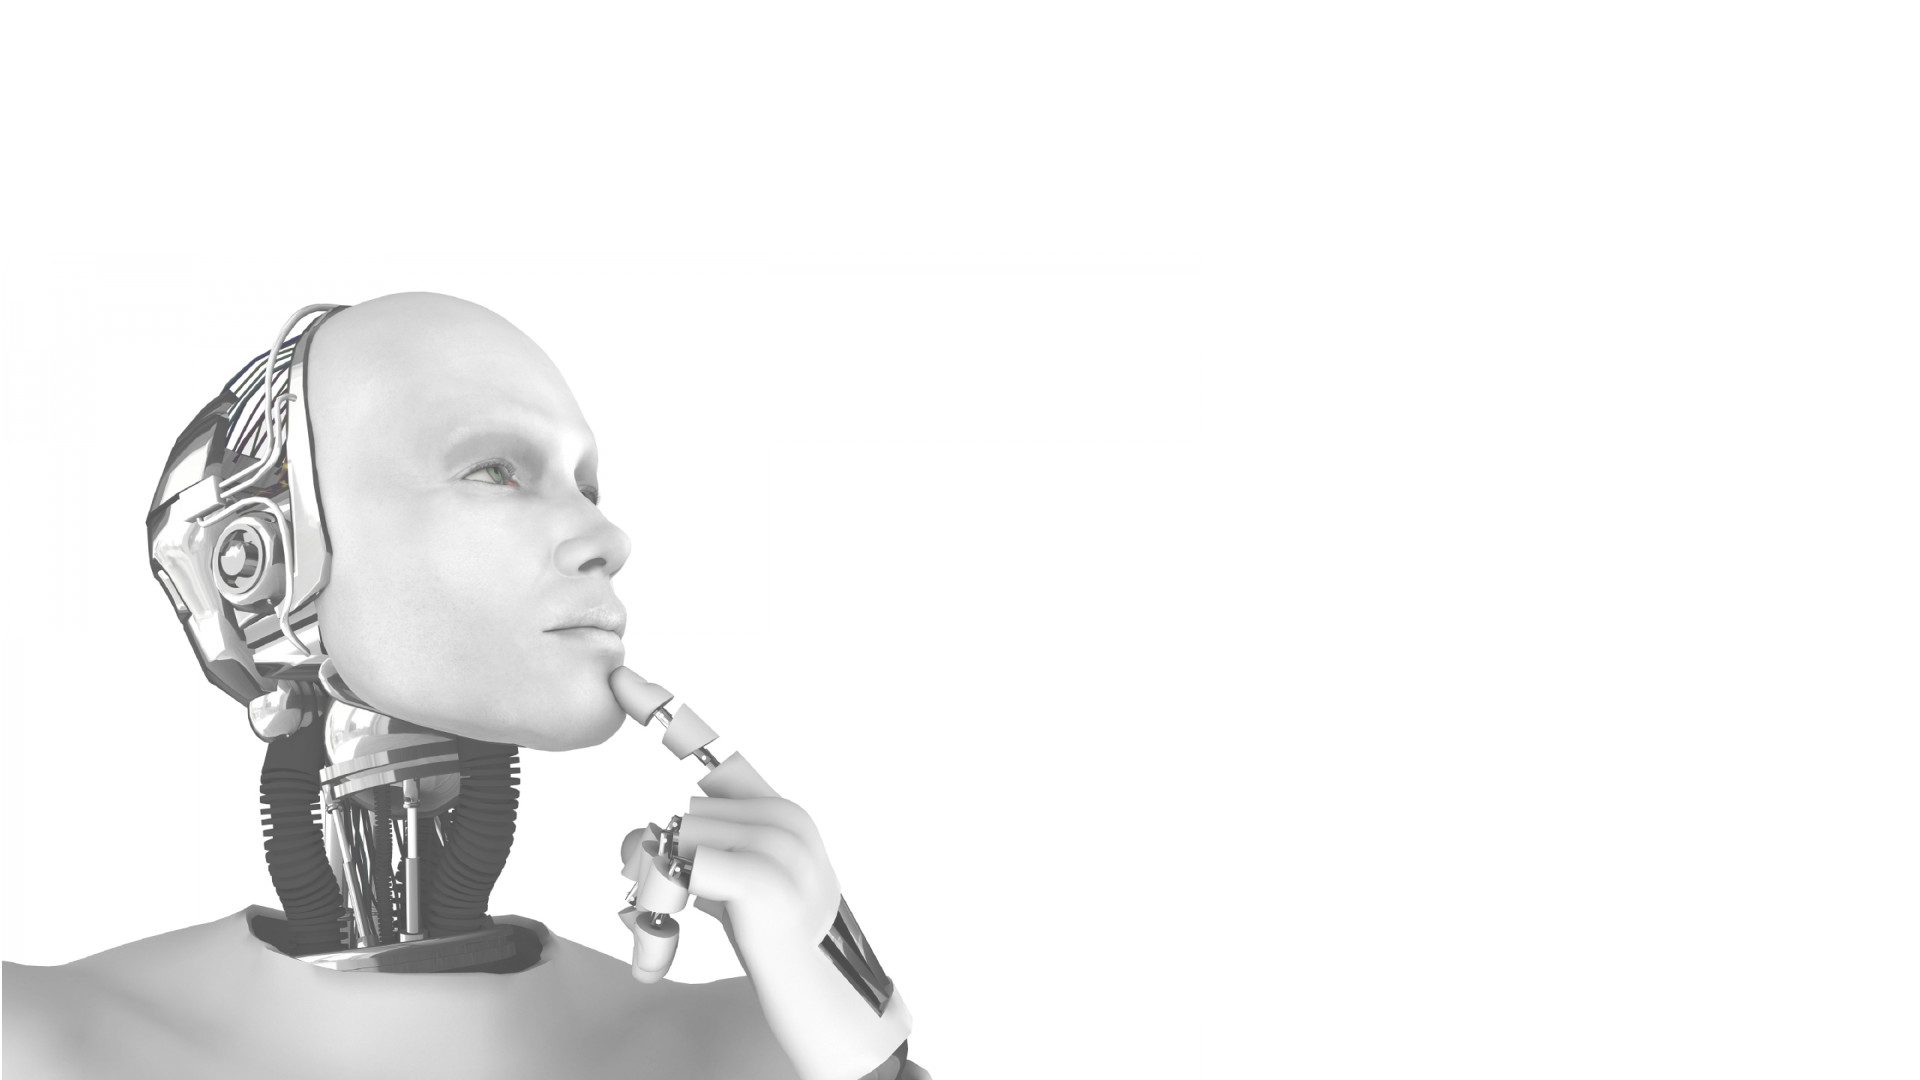
\includegraphics[width=\paperwidth]{images/ai_bg.jpg}}
\maketitle}

%\usebackgroundtemplate{
%}

%%%%%%%%%%%%%%%%%%%%%%%%%%%%%%%%%%%%%%%%%%%%%%%%%%%%%%%%%%%%%%%%%%%%%%%%%%%%%%%%
%                       DEFINITIONS
%%%%%%%%%%%%%%%%%%%%%%%%%%%%%%%%%%%%%%%%%%%%%%%%%%%%%%%%%%%%%%%%%%%%%%%%%%%%%%%%
%\section{SciFi debunked - Slaugherbots}
	\begin{frame}{Agenda}
		\tableofcontents

%	    \begin{itemize}
%		    \item Mission statement
%		    \item Get to know each other
%		    \item What is AI/ML?
%		    \item Presentations/Workshops for next session
%		    \item Open discussion
%	    \end{itemize}
	\end{frame}


\section{Slaugherbots}
        \begin{frame}{Video - Slaughterbots (7:47)}
        	\centering
        	Video released by autonomousweapons.org, shall support the campaign(s) to pass laws against autonomous weapons (https://www.stopkillerrobots.org/)
		In the video: Prof. Stuart Russel (AI/CompSci, UC Berkeley)

            {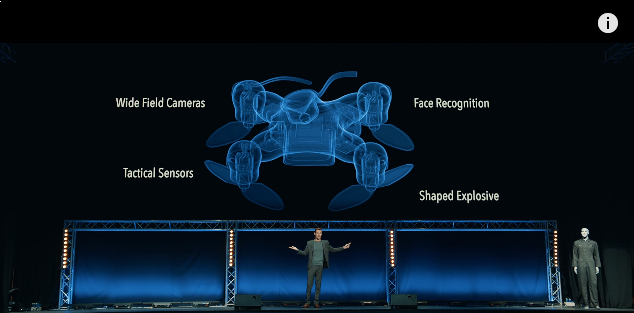
\includegraphics[width=.8\linewidth]{images/slaughterbots.png}}
        \end{frame}

        \begin{frame}{Video - Slaughterbots (7:47)}
        	\centering
            \href{run:./videos/Slaughterbots.mp4?autostart}
            {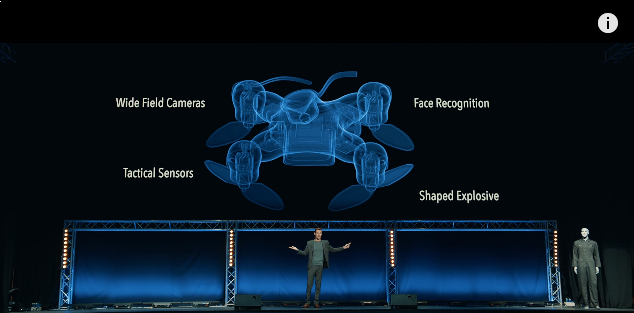
\includegraphics[width=1\linewidth]{images/slaughterbots.png}}
        \end{frame}

\section{Drone technology background}
\begin{frame}{Drone tech}
	\begin{figure}
		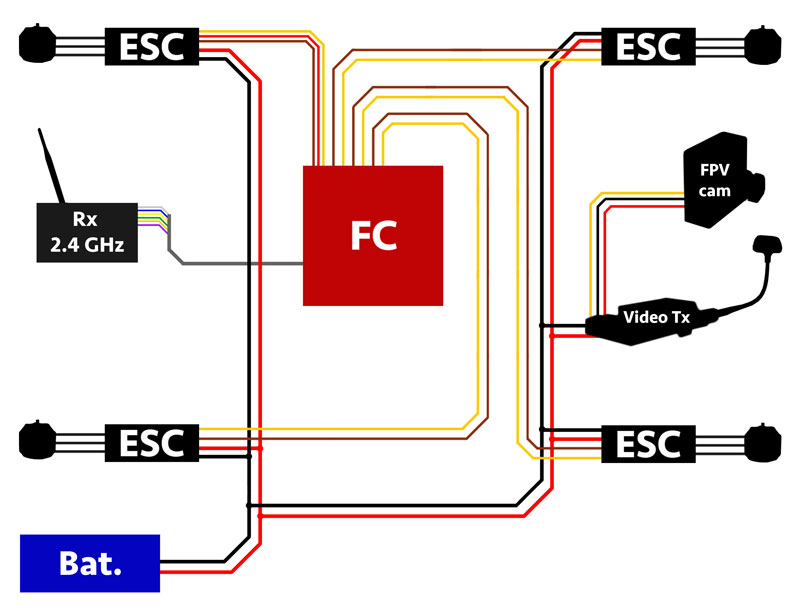
\includegraphics[width=0.6\linewidth]{images/06-FPV-Overview_1.jpg}
	\end{figure}
	\color{gray}{http://fpvracing.ch/img/cms/infobereich/Bauanleitung/06-FPV-Overview\_1.jpg}
\end{frame}

\begin{frame}{Drone tech - Hardware}
	\begin{figure}
		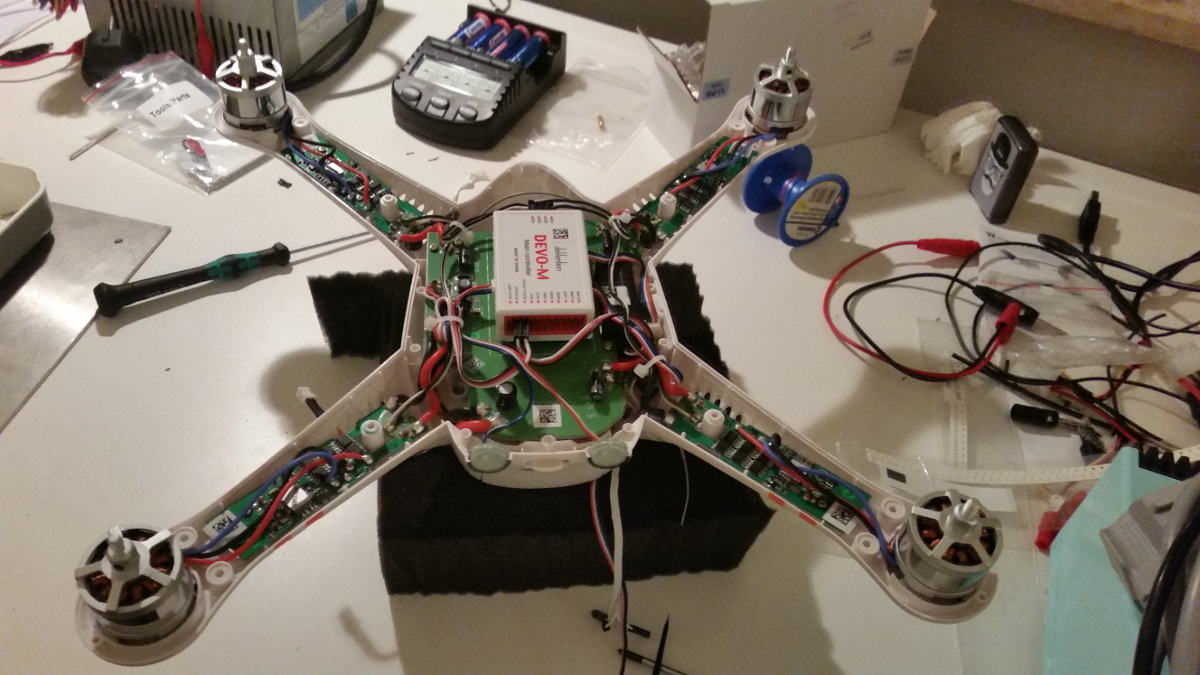
\includegraphics[width=0.9\linewidth]{images/qrx350pro_disassembled.jpg}
	\end{figure}
\end{frame}

\begin{frame}{Drone tech}
	Example: Walkera QR-X350 Pro
	\begin{itemize}
		\item Battery: 5Ah 30C Li-Po $\rightarrow$ 10-20 min. of flight w/ Cam + GPS
		\item Weight (incl. gimbal, camera, battery, transmitter): 1250g
		\item Topspeed: 71 km/h
		\item Cost: ca. 400 EUR
	\end{itemize}
	
	Remote-control
	\begin{itemize}
		\item Devo-7: 2.4Ghz, output: up to 20db (100mW) - up to 3km range
	\end{itemize}
	
	FPV - Camera stream transmission
	\begin{itemize}
		\item 5.8 Ghz transmitter, 600mw - up to 2km range, most often below 600m
	\end{itemize}
	
	Telemetry - Serial data connection
	\begin{itemize}
		\item 433 Mhz - more than 1km range
	\end{itemize}
\end{frame}

\begin{frame}{Drone tech - Sensors}
	To maintain stability and navigate, the Flight Controller is usually connected to a lot of onboard sensors:
	\begin{columns}
	\begin{column}{.8\textwidth}
	\begin{itemize}
		\item Acceleration/Turnrate: Accelerometer + Gyroscope
		
		\item Height: Barometer
		
		\item Global orientation: Magnetometer (Compass)
		
		\item Global positioning: GPS
		
		\item Relative speed: Optical flow

	\end{itemize}
	\end{column}
	
	\begin{column}{.19\textwidth}
		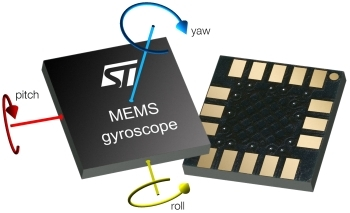
\includegraphics[width=0.8\linewidth]{images/acc_gyro.jpg}\\
		\vspace{0.2cm}
		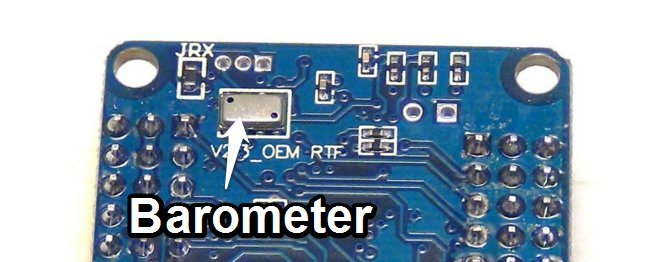
\includegraphics[width=0.8\linewidth]{images/barometer.jpg}\\	
		\vspace{0.2cm}	
		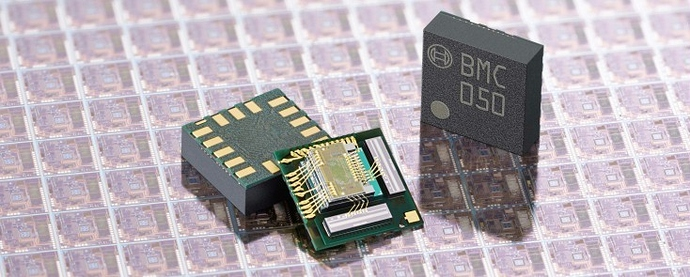
\includegraphics[width=0.8\linewidth]{images/magnetometer.jpg}\\
		\vspace{0.2cm}			
		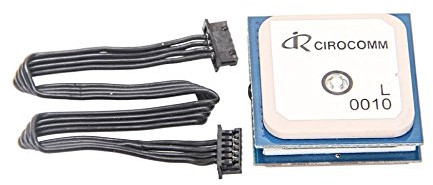
\includegraphics[width=0.8\linewidth]{images/cyrocomm_gps.jpg}\\
		\vspace{0.2cm}			
		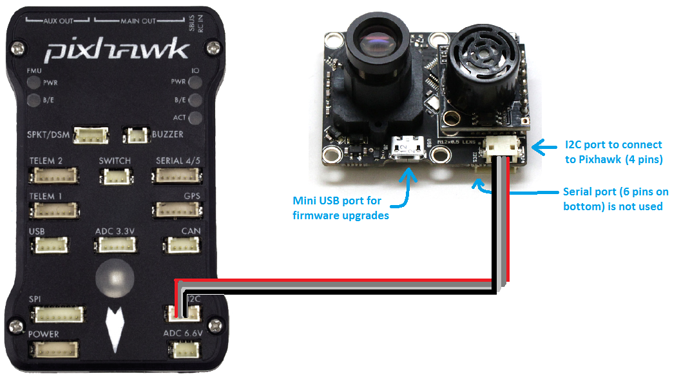
\includegraphics[width=0.8\linewidth]{images/optical_flow.png}	
	\end{column}
	\end{columns}
	\tiny{\color{gray}{Images from: http://www.dronetrest.com/t/beginners-guide-to-drone-autopilots-flight-controllers-and-how-they-work/1380}}
\end{frame}


\begin{frame}{Drone tech - GPS and positioning}
	\begin{columns}
	
	\begin{column}{.25\textwidth}
	\begin{figure}
		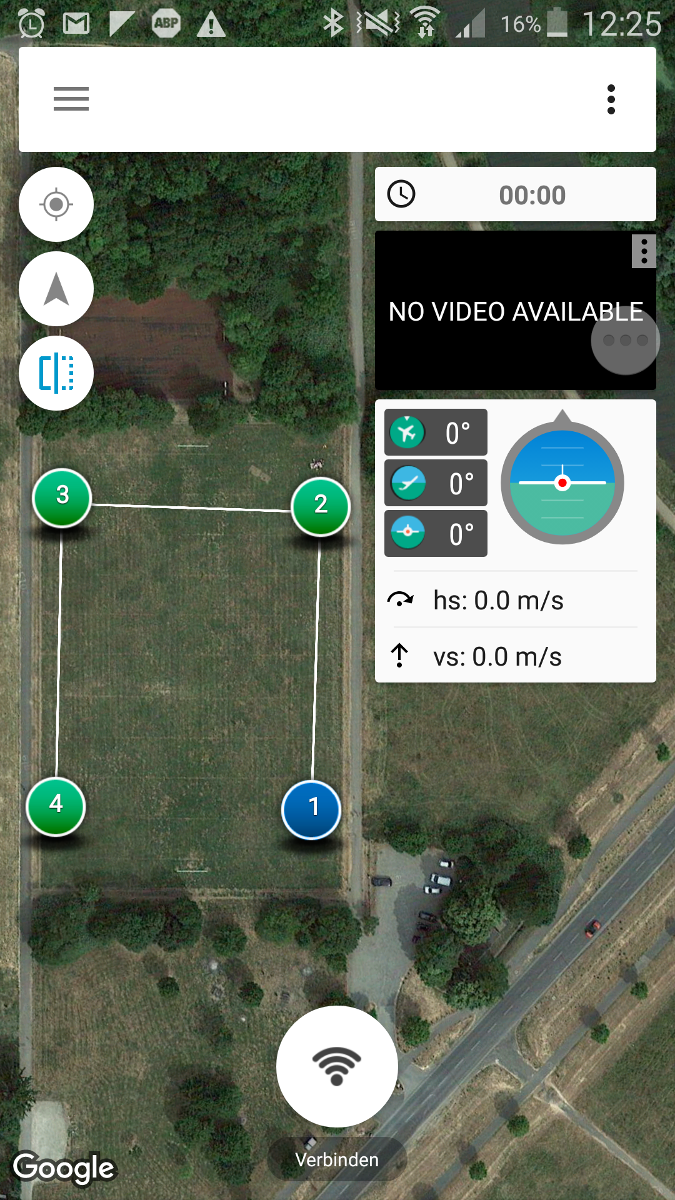
\includegraphics[width=1\linewidth]{images/qrx350pro_3drcontrol.png}\\
		\color{gray}{Tower android app}
	\end{figure}
	\end{column}
	
	\begin{column}{.74\textwidth}
		\begin{itemize}
			\item Mavlink-protocol to communicate with FlightController
			\item Get telemetry-data (current position, angles, height)
			\item Set targets, send control instructions
		\end{itemize}
	\end{column}
	
	\end{columns}
\end{frame}


%%%%%%%%%%%%%%%%%%%%%%%%%%%%%%%%%%%%%%%%%%%%%%%%%%%%%%%%%%
%%
%%%%%%%%%%%%%%%%%%%%%%%%%%%%%%%%%%%%%%%%%%%%%%%%%%%%%%%%%%
\section{Navigation, Localization and Control}

\begin{frame}{Navigation, localization and control}
	\begin{itemize}
		\item How are drones controlled at the moment?
		\item How can they navigate without crashing?
		\item What are the drawbacks?
		\item What are the current approaches to more autonomy?
	\end{itemize}
\end{frame}

\begin{frame}{Drone- and weapon-related science and projects}
	\begin{itemize}
		\item DoD: Perdix micro-drone-swarm
		%\item Israel Aerospace Industries: 
		%\item No Info about localization found: ETH Zurich (D'Andrea): http://flyingmachinearena.org/research/, https://www.youtube.com/watch?v=RCXGpEmFbOw
        \item The pentagon wants you to develop drone swarms: https://thenextweb.com/insider/2017/10/23/the-pentagon-wants-you-to-develop-drone-swarms-for-the-military/
	\end{itemize}
\end{frame}

\begin{frame}{Intel drone swarm}
        	\centering
            \href{run:./videos/Intel.mp4?autostart}
            {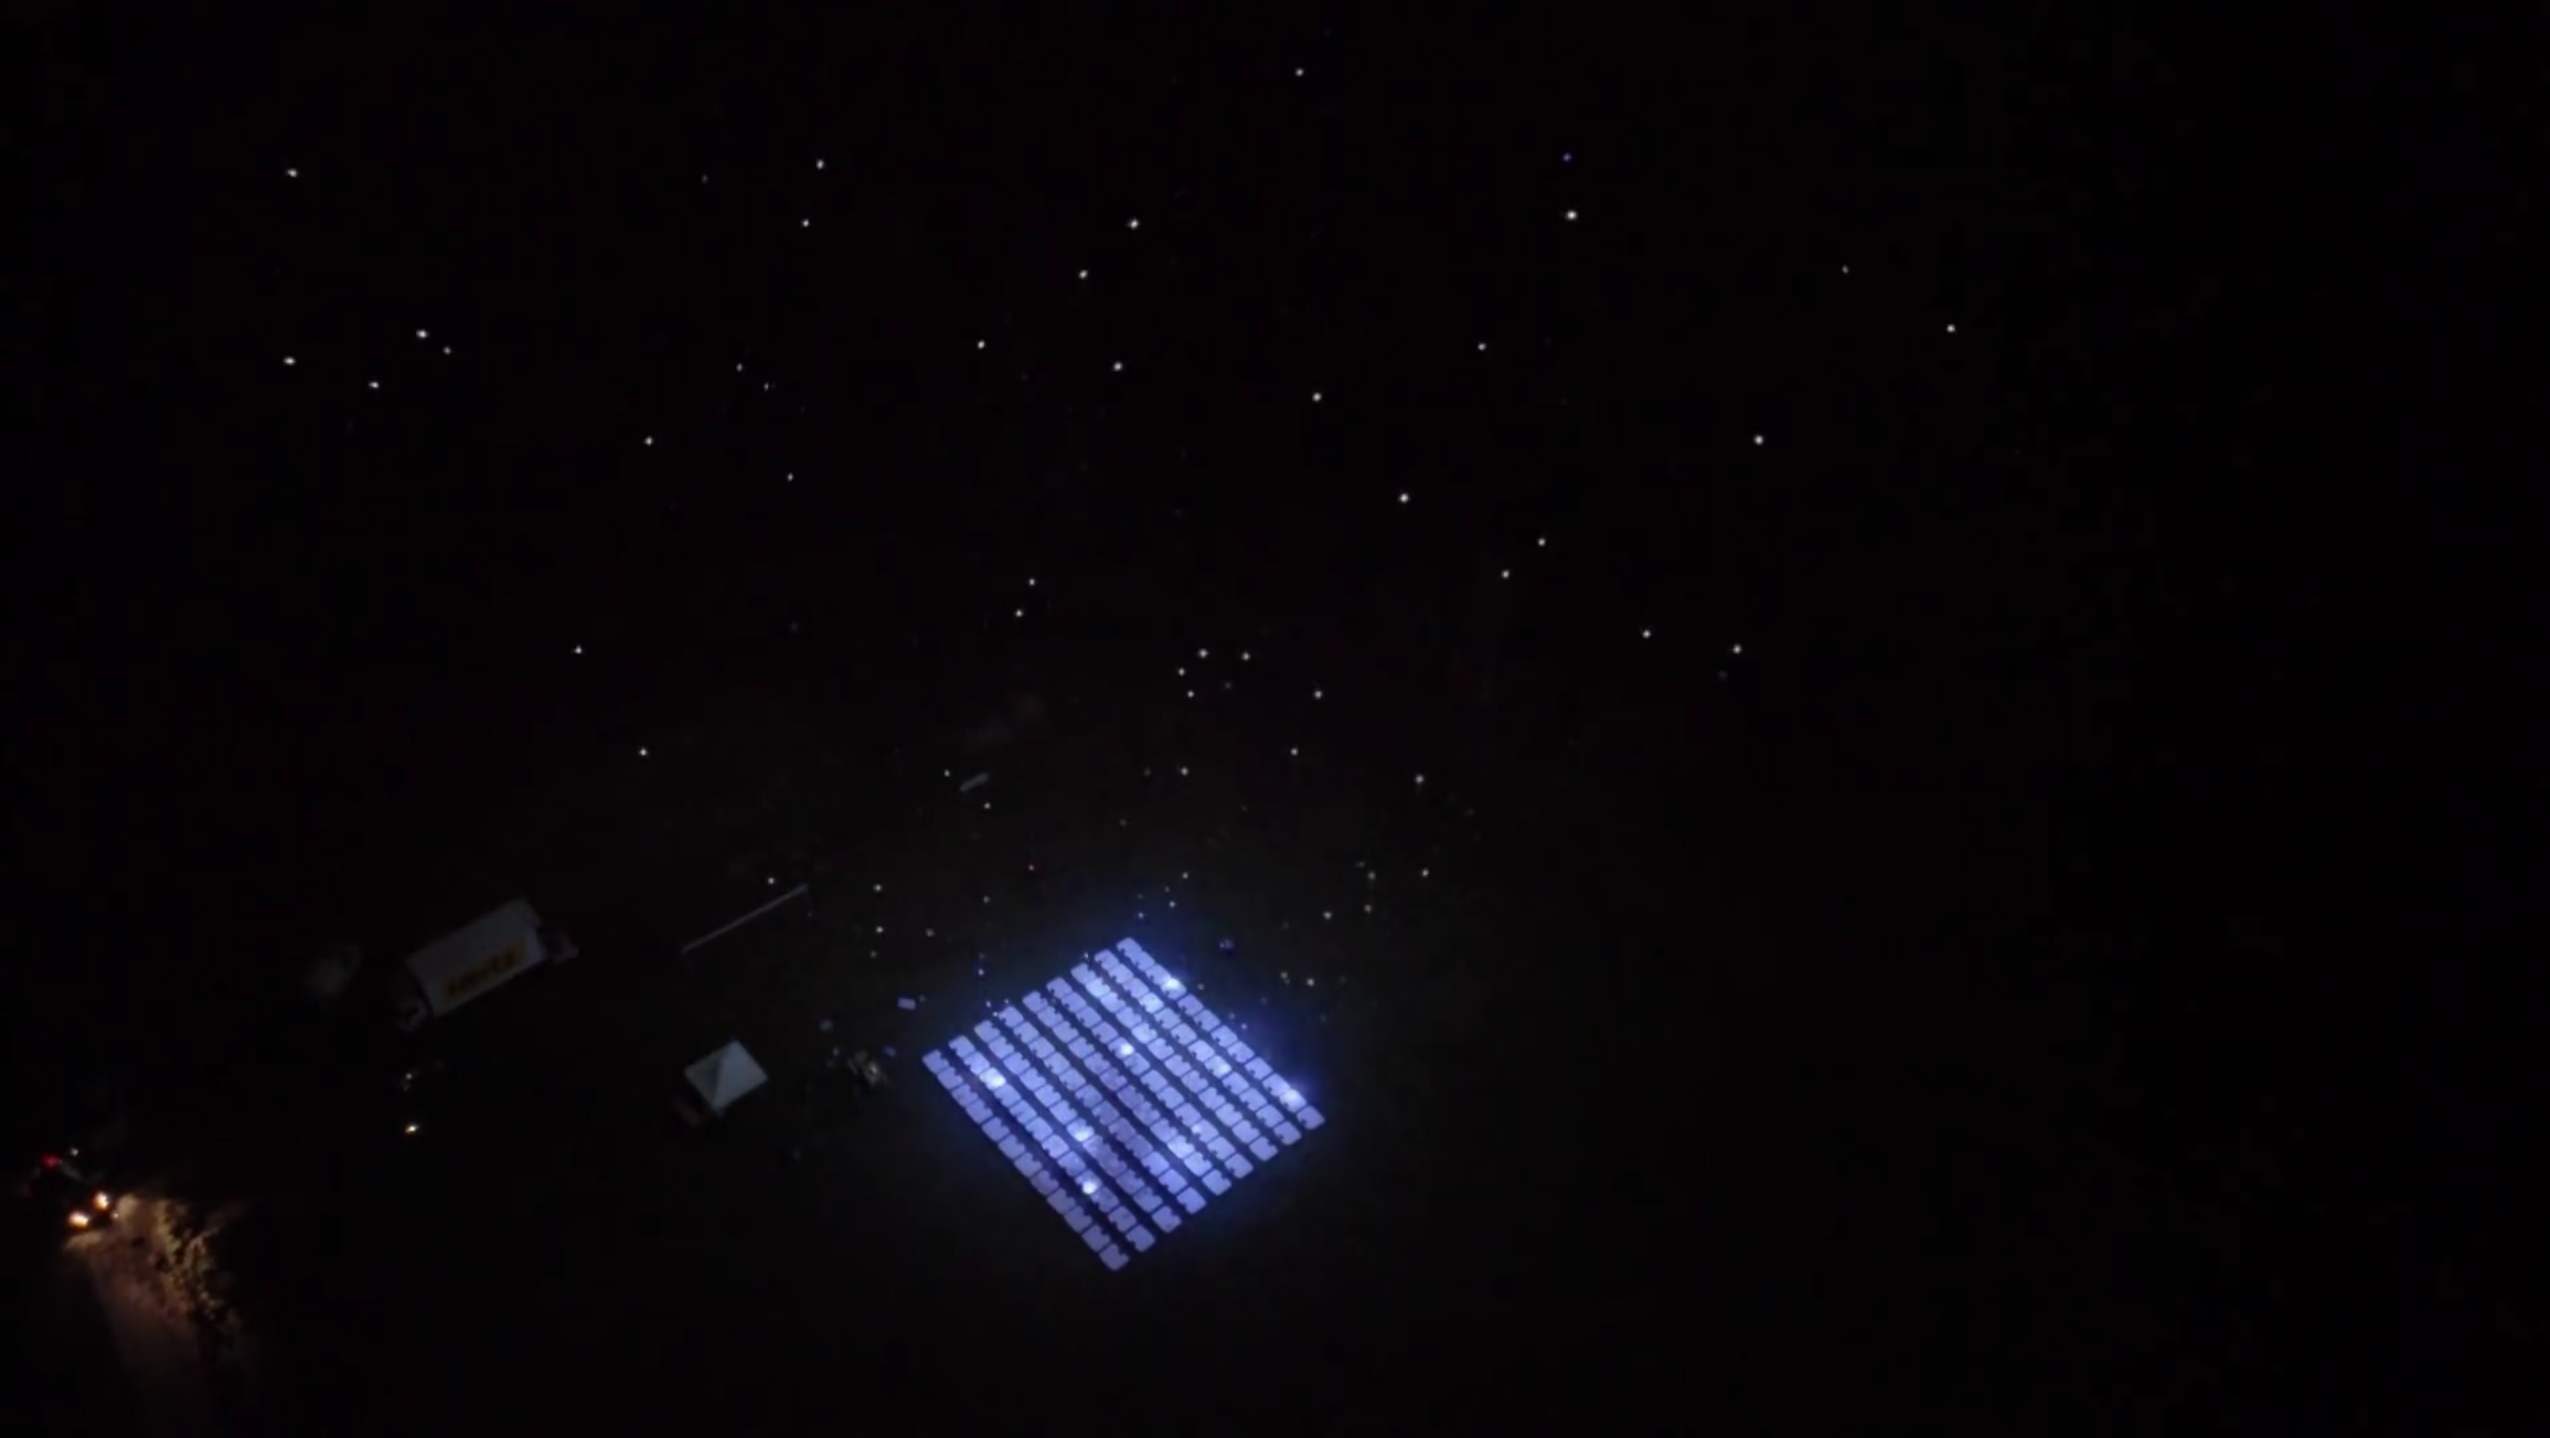
\includegraphics[width=.95\linewidth]{images/intel.png}}
           
\end{frame}


\begin{frame}{Intel drone swarm}
	\begin{columns}
	\begin{column}{0.6\textwidth}
	Intel's name of the drones used: Shooting Star
	\centering
	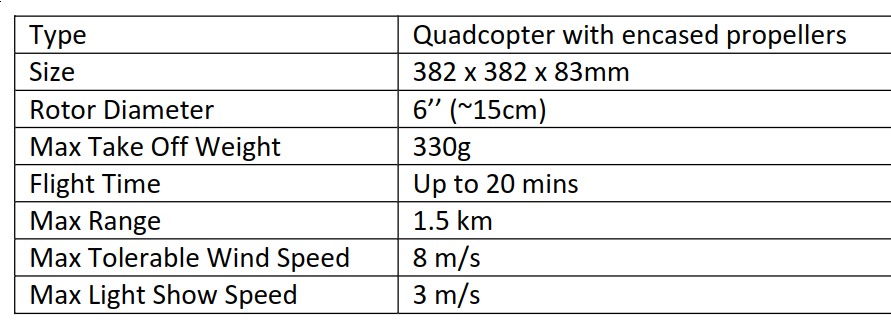
\includegraphics[width=\linewidth]{images/intel_shooting_star_specs.png}
	\begin{itemize}
		\item Relies on GPS (plus the other sensors you have already seen)
		\item Central control software on offboard computer
	\end{itemize}
	\end{column}
	
	\begin{column}{0.39\textwidth}
		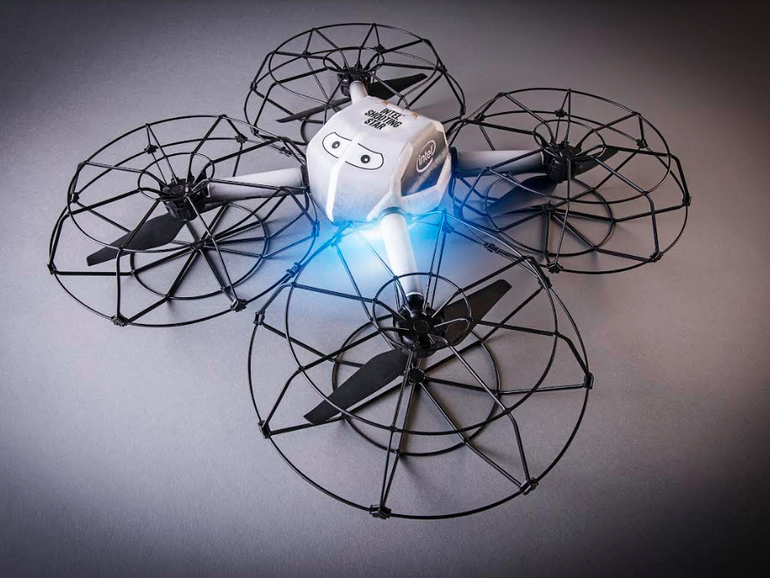
\includegraphics[width=\textwidth]{images/intel_shooting_star.png}
	\end{column}
	\end{columns}
	
	\vspace{10mm}
\tiny{\color{gray}{https://newsroom.intel.com/wp-content/uploads/sites/11/2017/07/Intel-Shooting-Star-Tech-Fact-Sheet-073117-1.pdf}}
\end{frame}

\begin{frame}{D'Andrea, ETH + Verity studios}
        	\centering
            \href{run:./videos/DAndre_TED_talk.mp4?autostart}
            {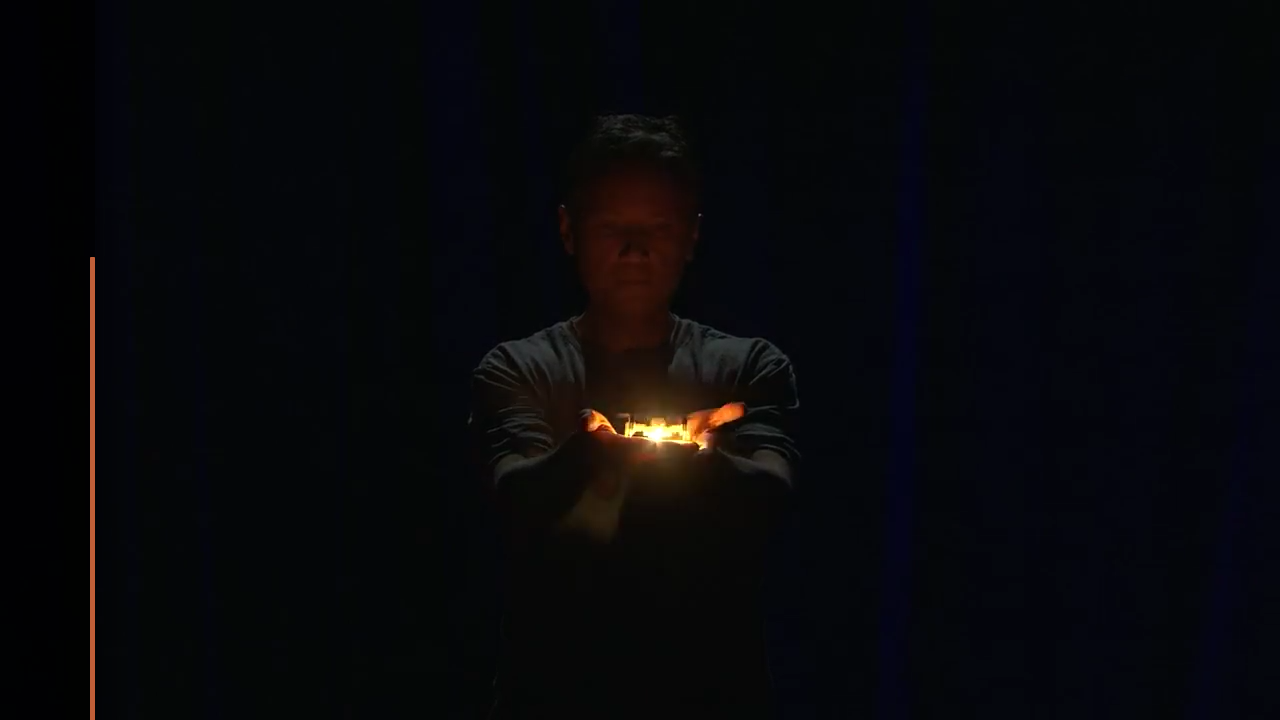
\includegraphics[width=.95\linewidth]{images/DAndre_TED_talk.png}}
\end{frame}

\begin{frame}{D'Andrea, ETH + Verity studios}
\begin{itemize}
	\item ETH-spinoff Verity studios
	\item No details about indoor-localization to be found, but:
\end{itemize}
\begin{columns}
\begin{column}{0.49\textwidth}
	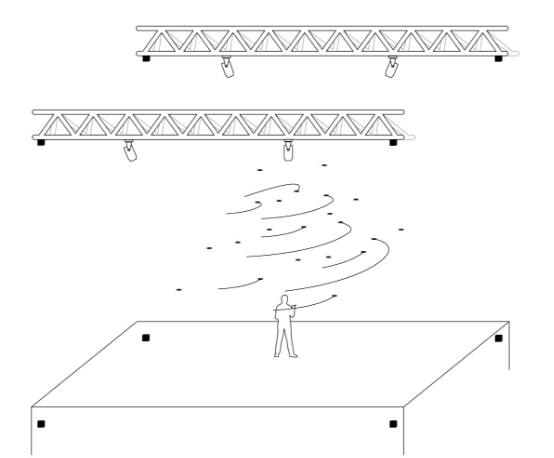
\includegraphics[width=\textwidth]{images/verity_loca.png}
\end{column}	
\begin{column}{0.49\textwidth}
	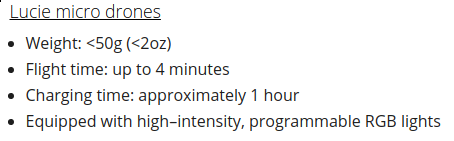
\includegraphics[width=\textwidth]{images/verity_specs.png}\\
		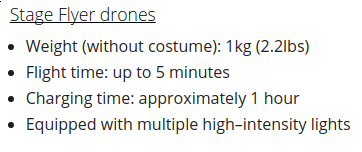
\includegraphics[width=\textwidth]{images/verity_specs2.png}
\end{column}
\end{columns}
\tiny{\color{gray}{https://veritystudios.com/products/\#synthetic-swarm}}
\end{frame}

\begin{frame}{Weaponized drones - Some guy (Austin Haghwout)}
\centering
            \href{run:./videos/flying_gun.mp4?autostart}
            {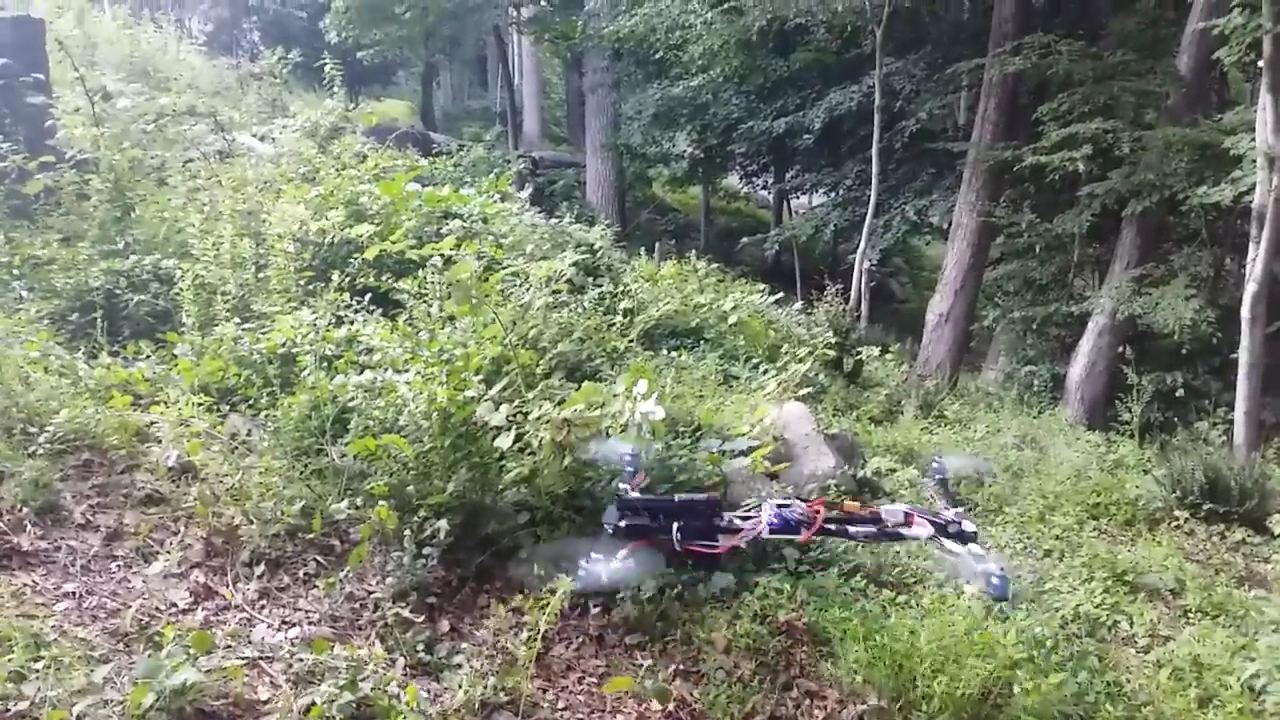
\includegraphics[width=.95\linewidth]{images/flying_gun.png}}
\end{frame}

\begin{frame}{Weaponized drones - IAI}
IAI - Israel Aerospace Industries\\
\begin{itemize}
	\item 4.5 kg,day/night cameras for piloting and reconnaissance
	\item multiple acoustic transducers (obstacle avoidance, flight through buildings)
	\item 30 minutes flight time with 0.45kg of explosive payload
	\item Warhead: two blast-fragmentation grenades
	\item packed folded, transported in canister or backpack
	\item piloted with tablet
\end{itemize}

\tiny{\color{gray}{http://defense-update.com/20160216\_rotem.html}}
\end{frame}

\begin{frame}{Weaponized drones - Duke Robotics}
\href{run:./videos/duke_robotics.mp4?autostart}
            {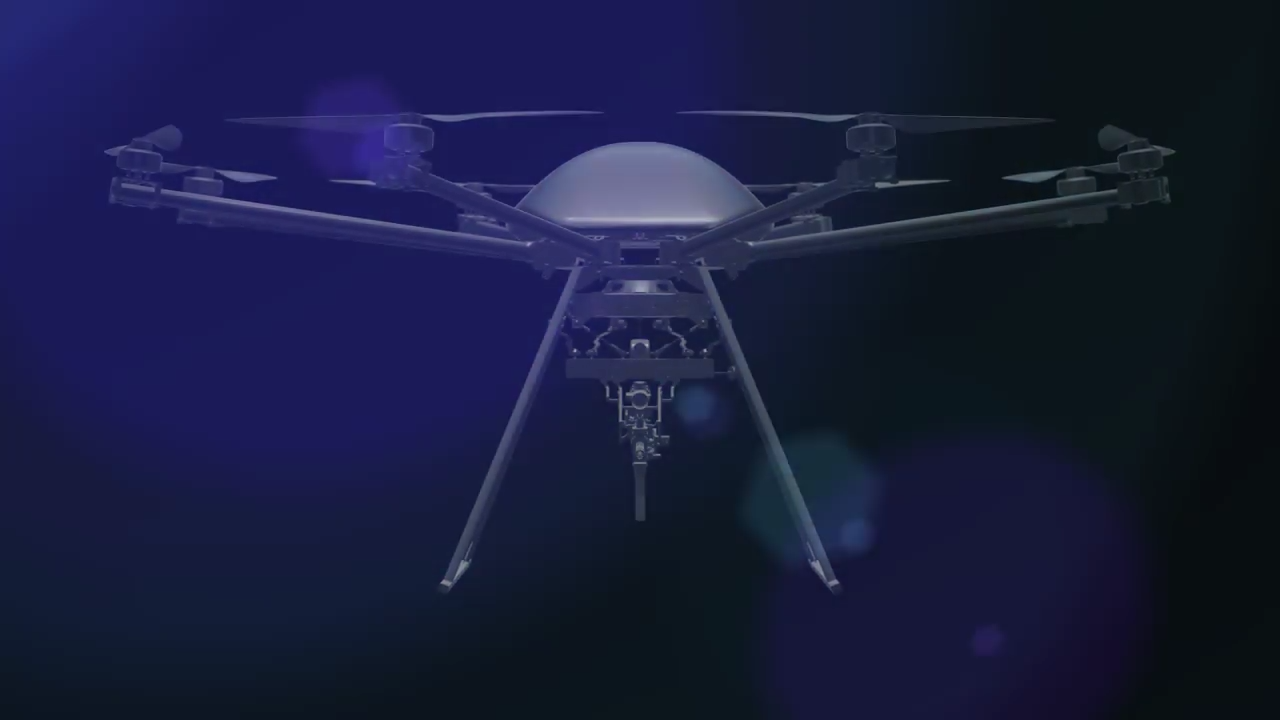
\includegraphics[width=.95\linewidth]{images/duke_robotics.png}}
\tiny{\color{gray}{https://dukeroboticsys.com/invest/}}
\end{frame}

\begin{frame}{How to defend?}
	Already, a lot of different ideas are tested to defend against drone attacks
\end{frame}

\begin{frame}{Weaponized drones - Countermeasures}
\centering
            \href{run:./videos/EaglesVsDrones.mp4?autostart}
            {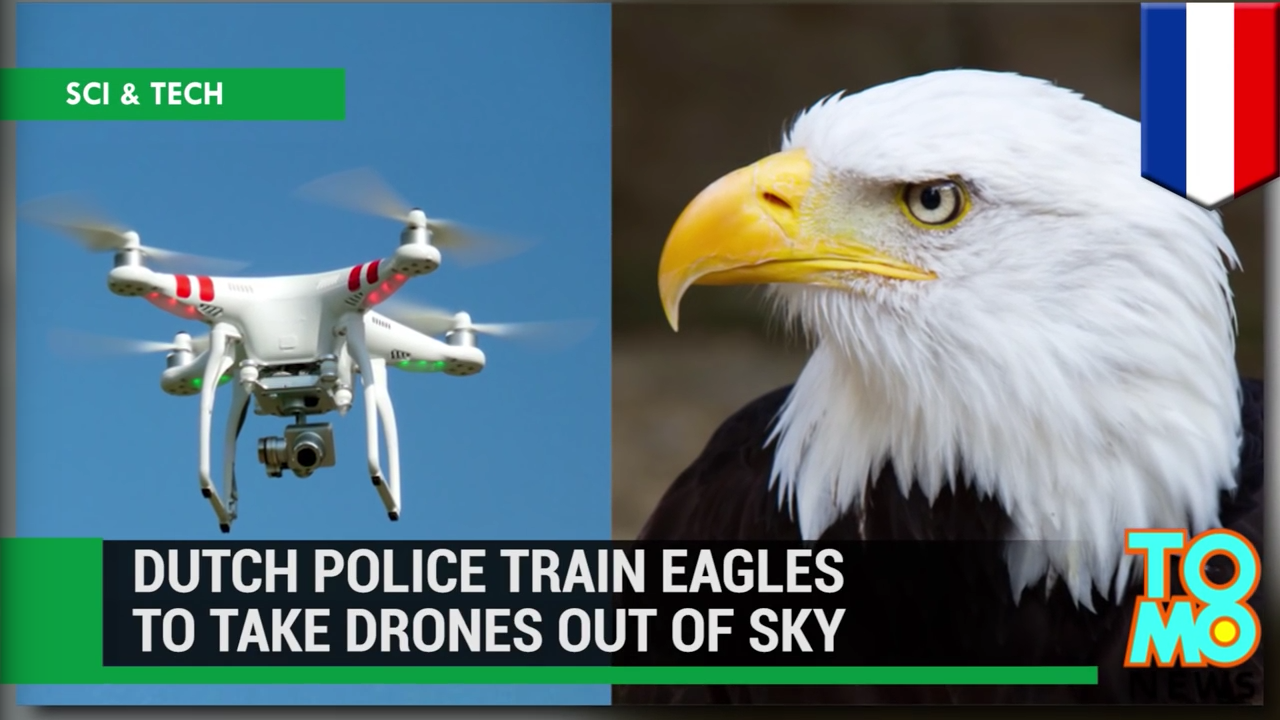
\includegraphics[width=.98\linewidth]{images/EaglesVsDrones.png}}
\end{frame}

\begin{frame}{Weaponized drones - Countermeasures}
\centering
            \href{run:./videos/SkyWall.mp4?autostart}
            {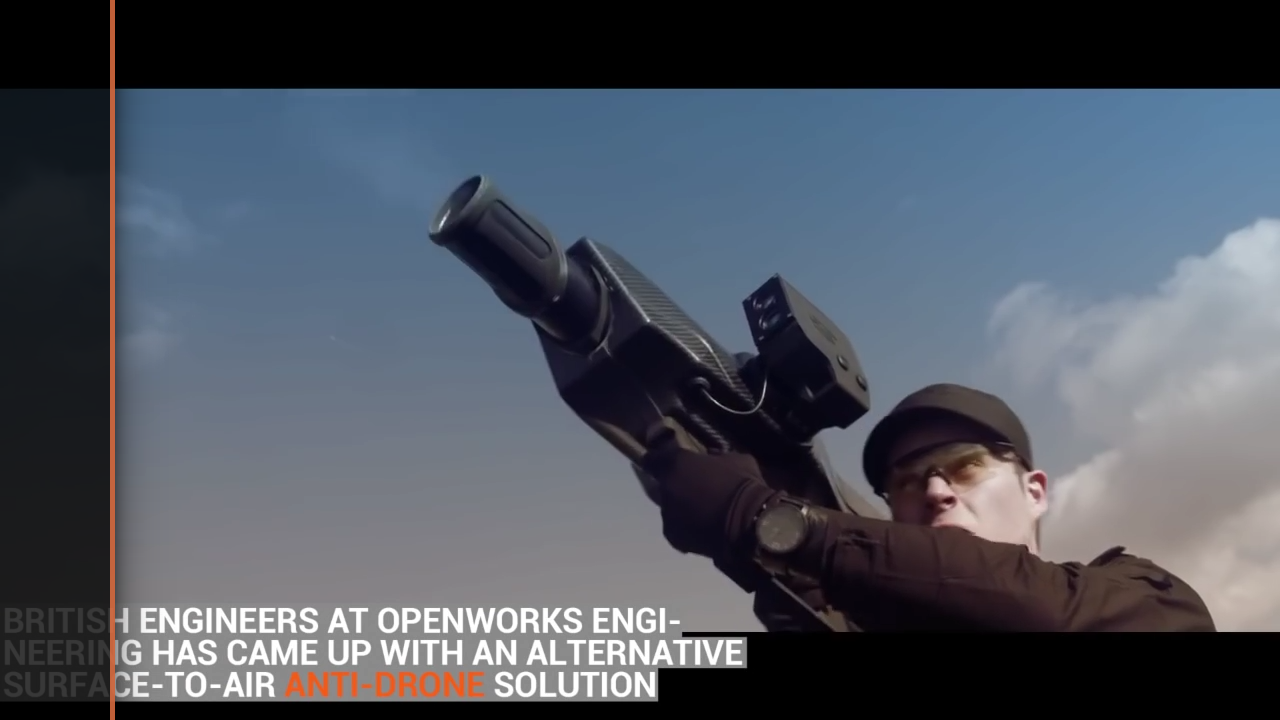
\includegraphics[width=.98\linewidth]{images/SkyWall.png}}
\end{frame}

\begin{frame}{Weaponized drones - Countermeasures}
\centering
            \href{run:./videos/DroneCatcher.mp4?autostart}
            {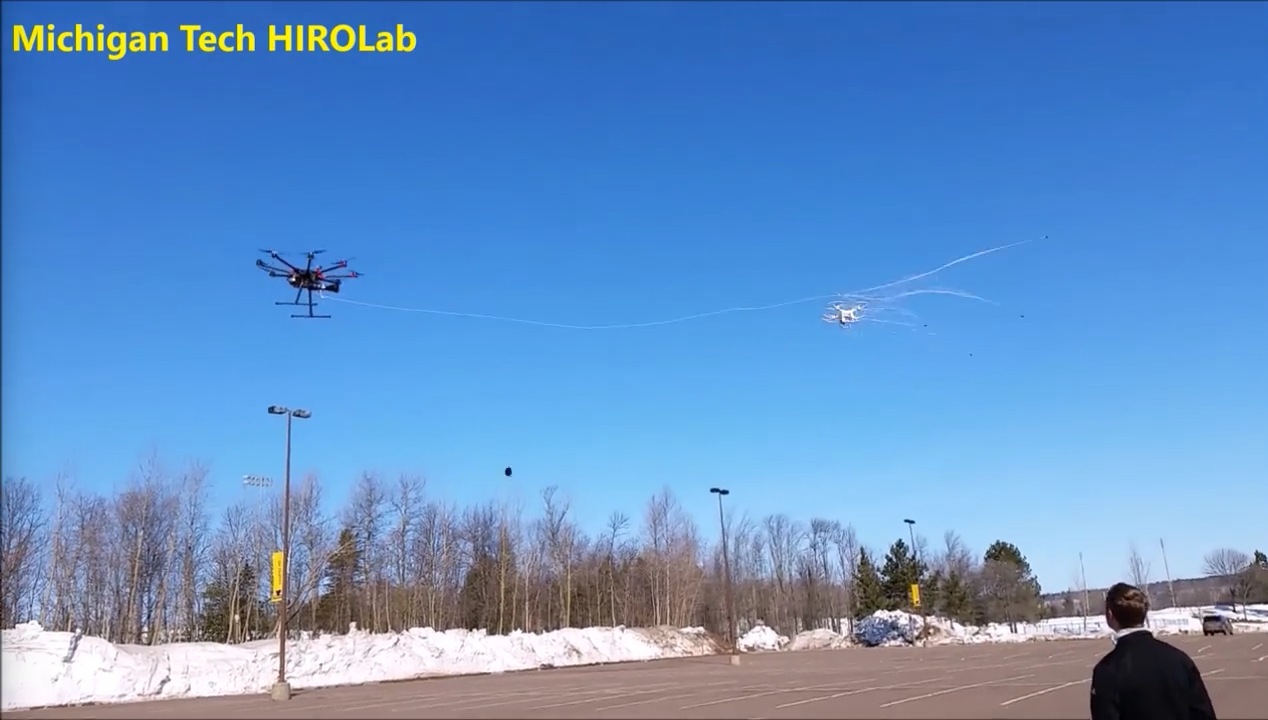
\includegraphics[width=.98\linewidth]{images/DroneCatcher.png}}
\end{frame}

\begin{frame}{Weaponized drones - Countermeasures}
\centering
            \href{run:./videos/LawsAntiDroneLaser.mp4?autostart}
            {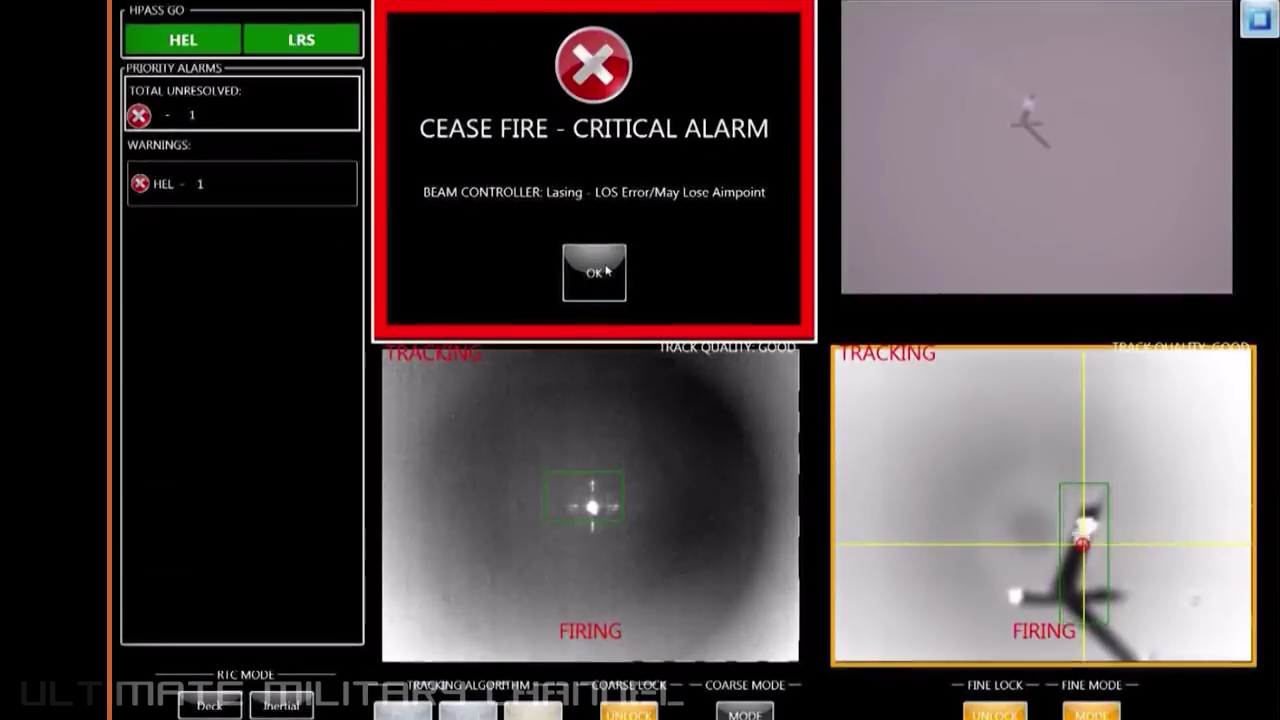
\includegraphics[width=.98\linewidth]{images/LawsAntiDroneLaser.png}}
\end{frame}

\begin{frame}{Weaponized drones - Countermeasures}
	Most of these approaches are expensive or not really feasible. The currently most often used approach is therefore:
	\begin{itemize}
		\item Jam signals by overpowering them with noise
		\item "Take out" GPS-positioning (1575.42 MHz or 1227.60 MHz) and radio remote-control (2.4Ghz)
	\end{itemize}

\centering
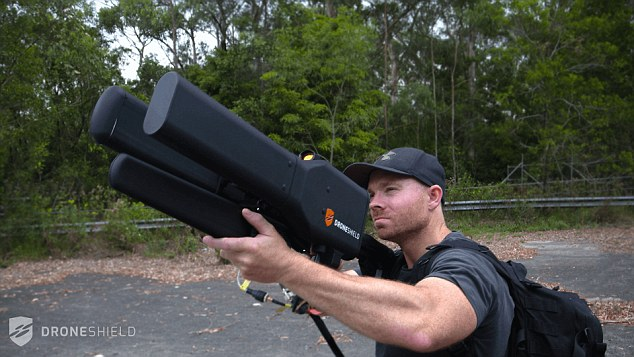
\includegraphics[width=.4\textwidth]{images/drone_jammer.jpg}
	\begin{itemize}
		\item Logical next step? Autonomy without GPS and remote operator.
	\end{itemize}

\tiny{\color{gray}{http://www.dailymail.co.uk/sciencetech/article-3978762/The-death-ray-knock-drones-mile-away-Rifle-uses-radio-waves-kill-UAVs.html}}
\end{frame}



\section{Autonomous drones}
\begin{frame}{Autonomy}
	Entering AI/ML: How can an artificial system perceive, act, localize and navigate in an unknown open world without a human operator?
	\begin{itemize}
		\item \textbf{Learn} from examples - Build knowledge - Abstract and apply
		\item For the weaponization scenario: Without sensors that might be jammed
	\end{itemize}
\end{frame}

\begin{frame}{NVIDIA - Autonomous Drone video (3:10)}
        	\centering
            \href{run:./videos/AutoDroneNvidia.mp4?autostart}
            {\includegraphics[width=\linewidth]{images/AutoDroneNvidia.png}}
\end{frame}

\begin{frame}{NVIDIA - Autonomous Drone video (3:10)}
	\begin{itemize}
		\item NVIDIA Jetson TX1 onboard processing, trained on videos of eight miles of trails
		%\item Sensors: PX4FLOW  optical  flow  sensor  with  sonar,and Lidar Lite V3.		
		\item Resnet-18 architecture computes view orientation and lateral offset output
		\item YOLO DNN for object detection, Visual odometry
		%\item Controller runs at 20Hz
		%\item Training data: videos shot along eight miles of trails in the Pacific Northwest, different lighting conditions with three wide-angle GoPro cameras mounted on the left, center and right of a metal bar on a mini Segway
	\end{itemize}
	\centering
	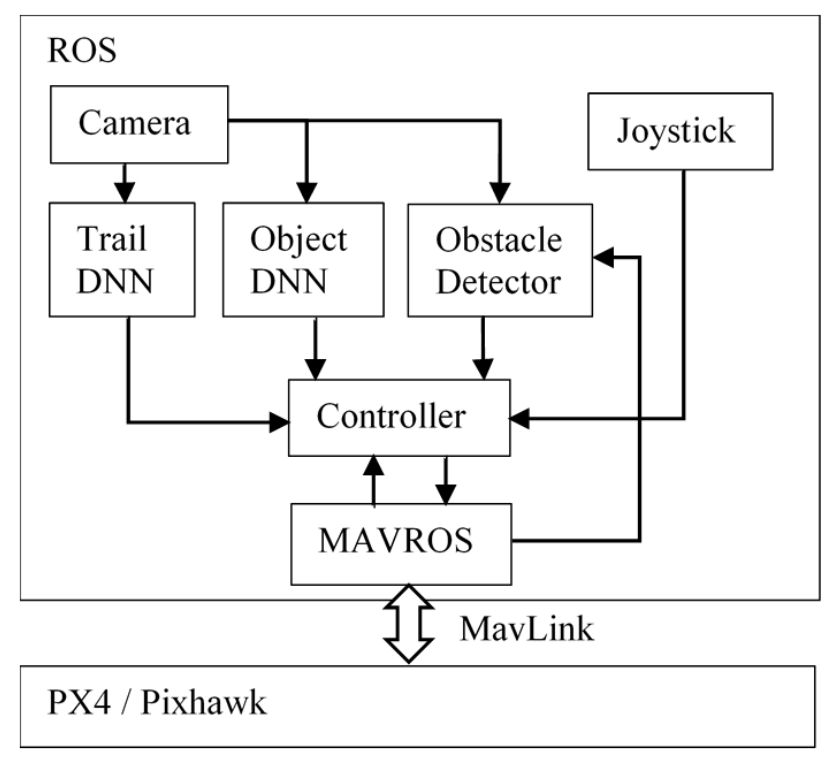
\includegraphics[width=.4\textwidth]{images/nvidia_controller.png}
	
	\tiny{\color{gray}{https://arxiv.org/pdf/1705.02550.pdf}}
	
\end{frame}

\begin{frame}{NASA JPL autonomous drone race}
        	\centering
            \href{run:./videos/NasaAutoDrone.mp4?autostart}
            {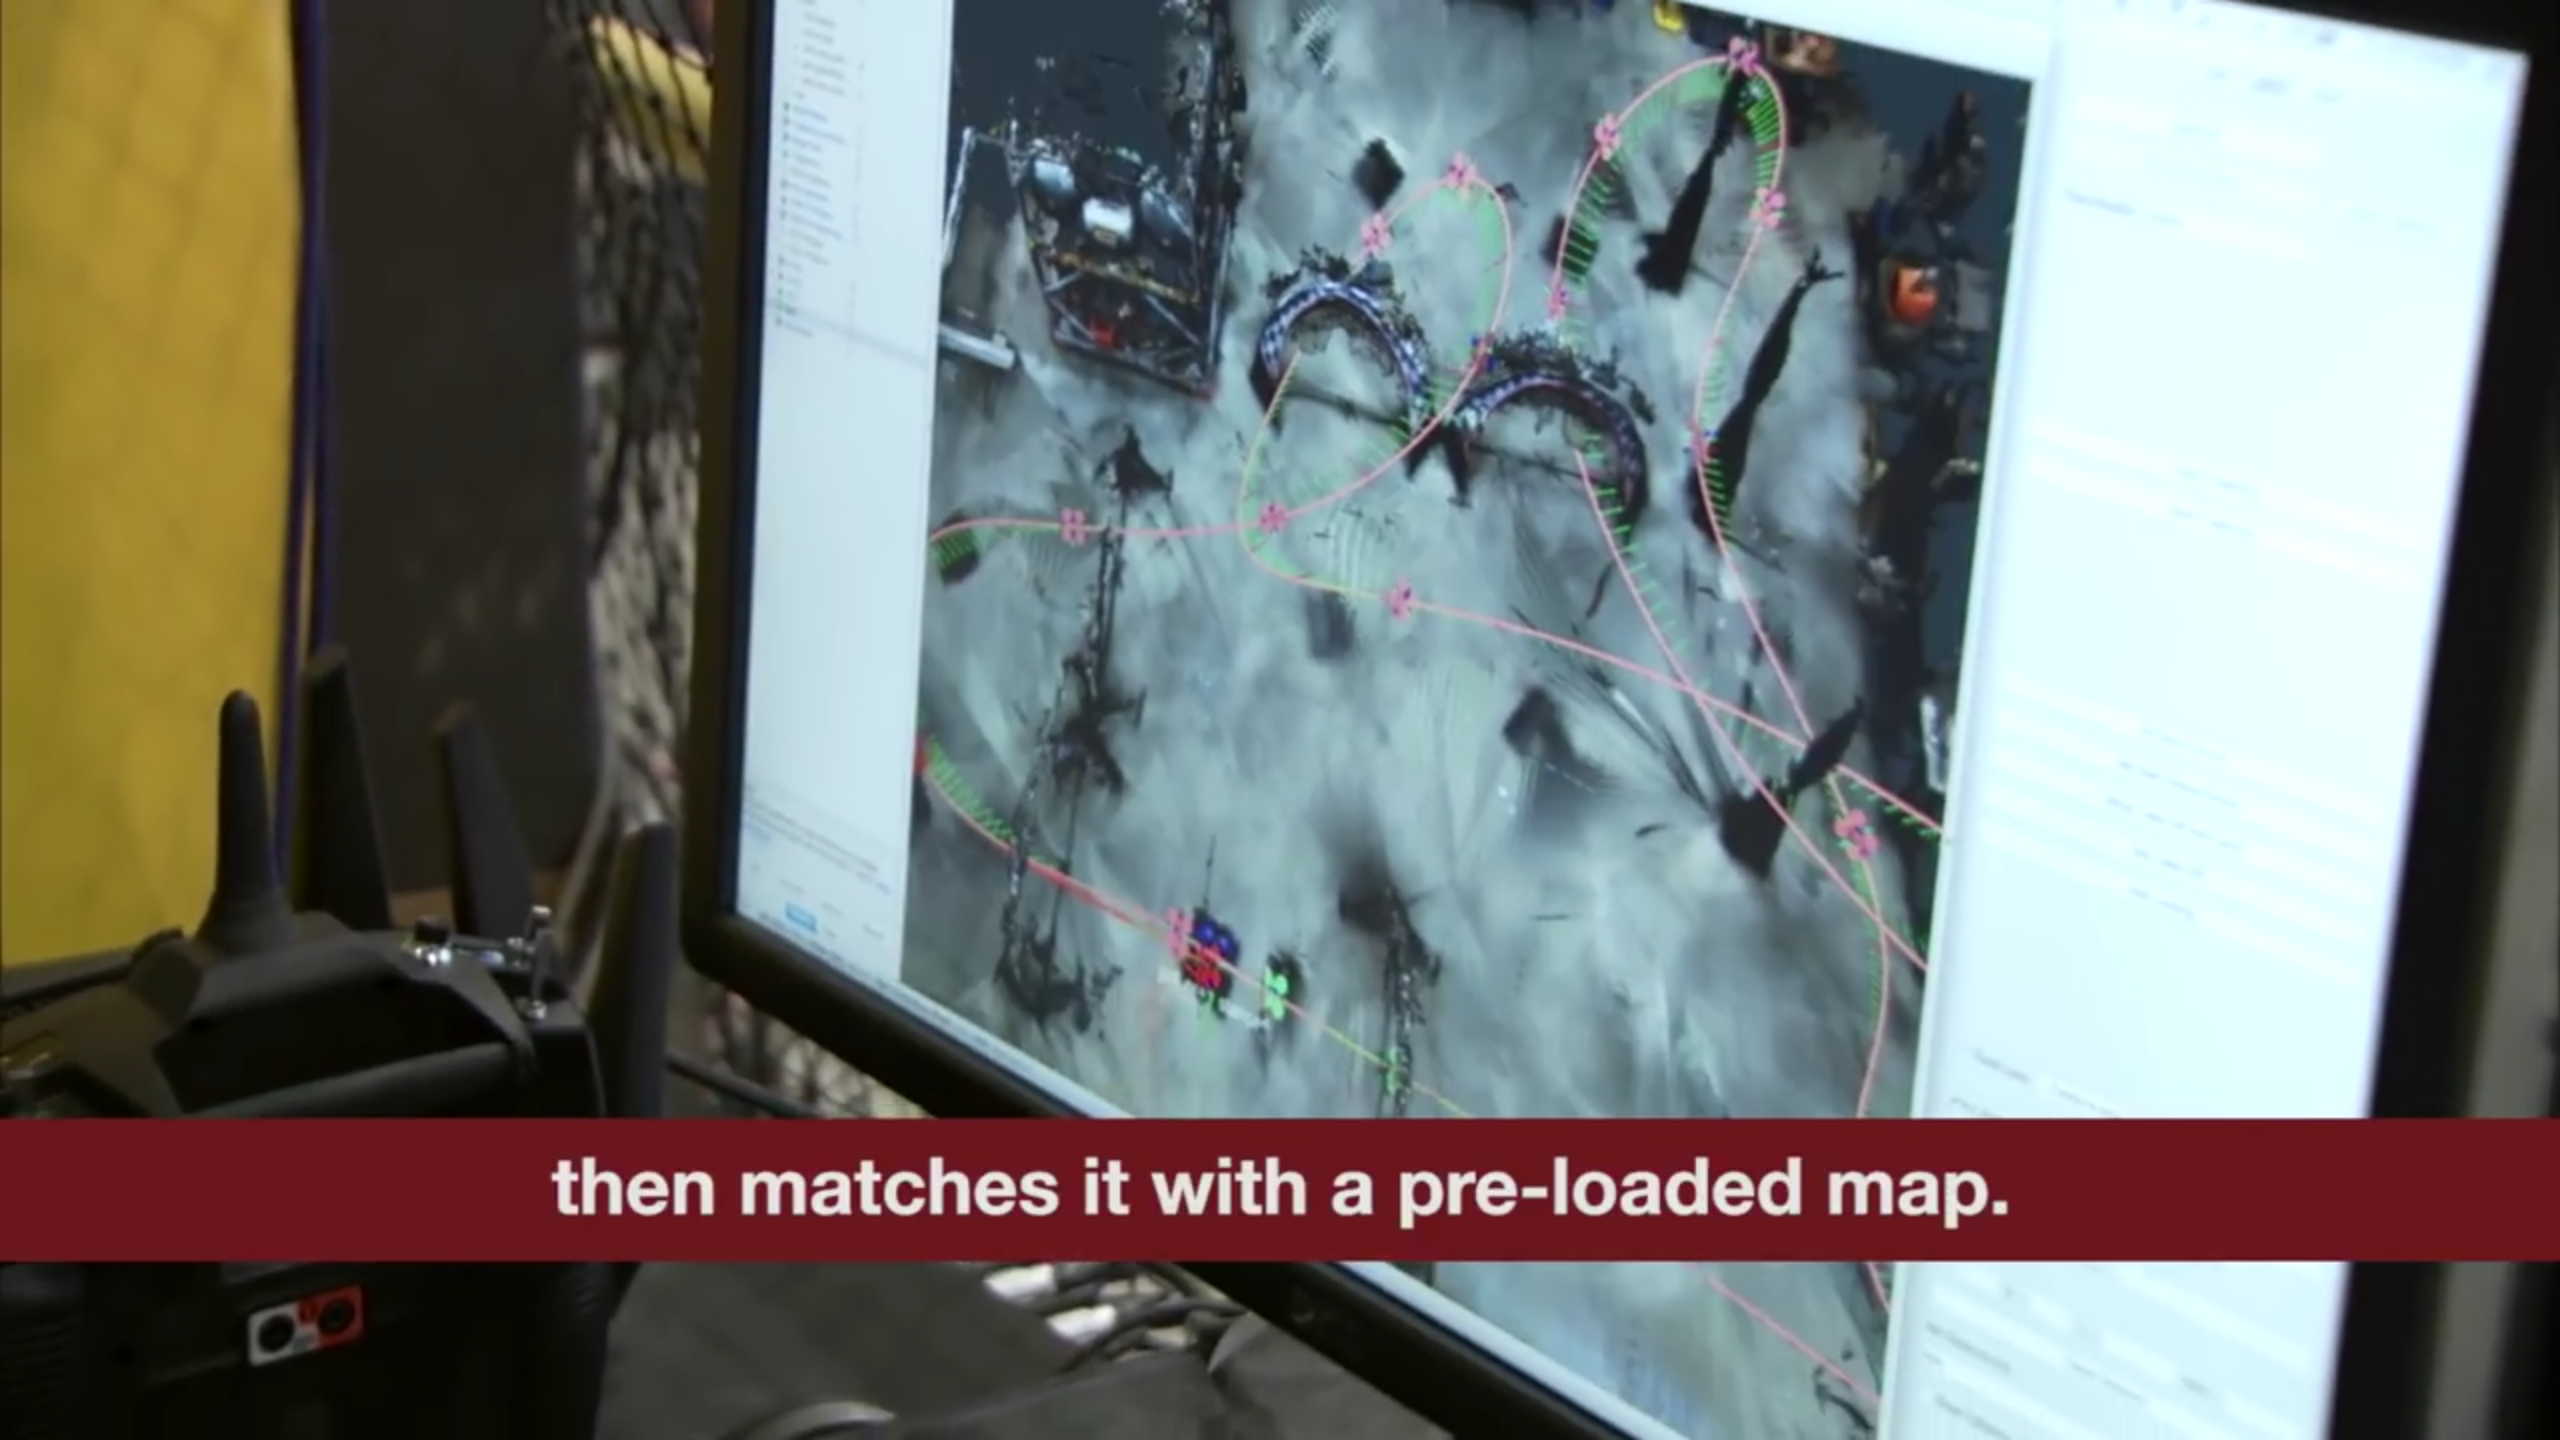
\includegraphics[width=\linewidth]{images/nasa.png}}
\end{frame}

\begin{frame}{NASA JPL autonomous drone race}
	\begin{quote}
		[...] processing is all done onboard. The team holds the drone and “walks” it through the course slowly ahead of the race to “teach” it the layout.[...] \hfill (Andrew Good, JPL, 06.12.17)
	\end{quote}

	\begin{columns}
	\begin{column}{.3\textwidth}
		\centering
		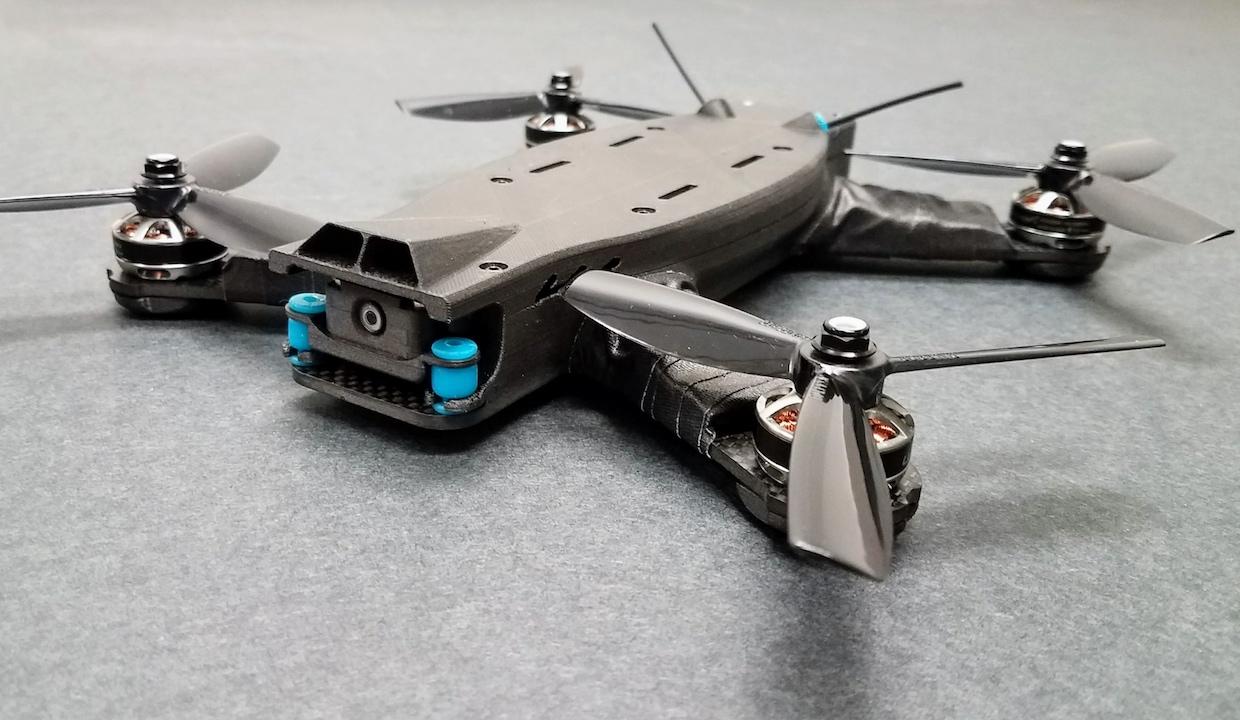
\includegraphics[width=\textwidth]{images/jpl_drone.jpeg}	
	\end{column}
	
	\begin{column}{.7\textwidth}
	\begin{itemize}
		\item Localize by comparing current sensor-input to pre-built map
		\item Google Tango technology for VR - 3D mapping
		\item Qualcomm Snapdragon Flight board is used for real-time flight control
		\item 2 wide-field-of-view-cameras: forward + downward
		\item Depth-map from motion stereo
	\end{itemize}
	\end{column}
	\end{columns}
	
	\vspace{5mm}
	\color{gray}{https://www.nasa.gov/feature/jpl/drone-race-human-versus-artificial-intelligence}
\end{frame}

\begin{frame}{UPENN - Vijay Kumar Lab - RAPID}
	\centering
            \href{run:./videos/kumar_lab.mp4?autostart}
            {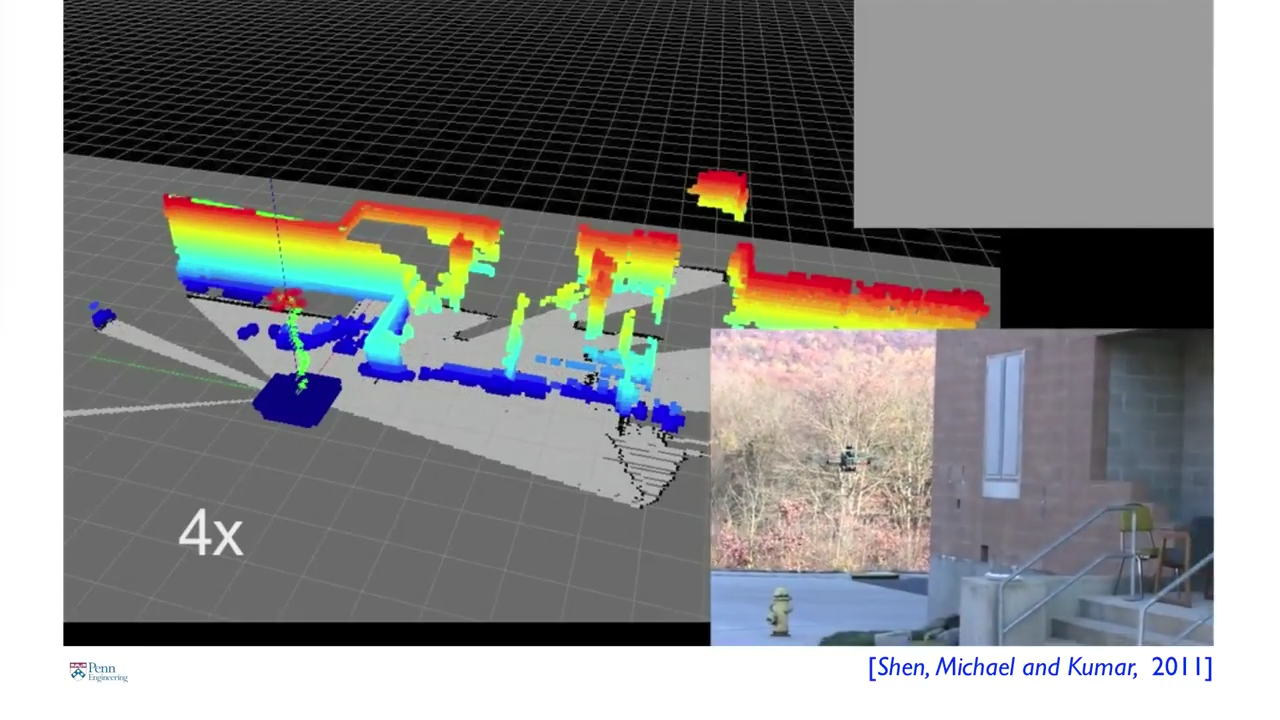
\includegraphics[width=.95\linewidth]{images/kumar_lab.png}}
\end{frame}

\begin{frame}{UPENN - Vijay Kumar Lab - RAPID}
	\begin{columns}
	
	\begin{column}{.49\textwidth}
	\begin{itemize}
		\item 1.9 kg MAV platform 
		\item IMU, laser scanner, stereo cameras, pressure altimeter, magnetometer, GPS 
		\item computation is performed onboard on an Intel NUC computer with 3rd generation i3 processor.
	\end{itemize}
	
	\end{column}
	\begin{column}{.49\textwidth}
	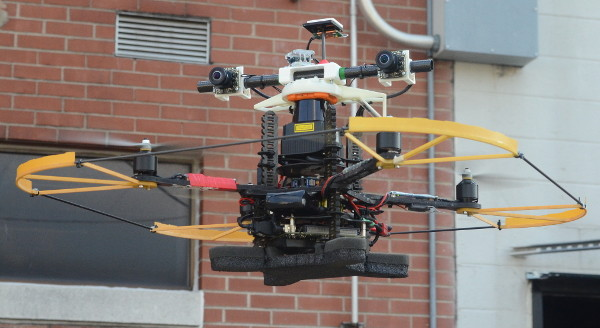
\includegraphics[width=\textwidth]{images/kumar_lab.jpg}
	\end{column}
	\end{columns}	
	\vspace{15mm}
	\color{gray}{https://www.kumarrobotics.org/videos/rapid/}
\end{frame}

\section{Finding and Identifying targets}
\begin{frame}{And now?}
	\begin{itemize}
		\item Drones are now able to fly without operator and without crashing
		\item How should they find their targets in the Slaughterbot scenario?
		\item State-of-the-art in ML allows to find human bodies in camera images (when sufficiently bright)
		\item The drone can attempt facial identification once a body is found		
	\end{itemize}
	\centering
	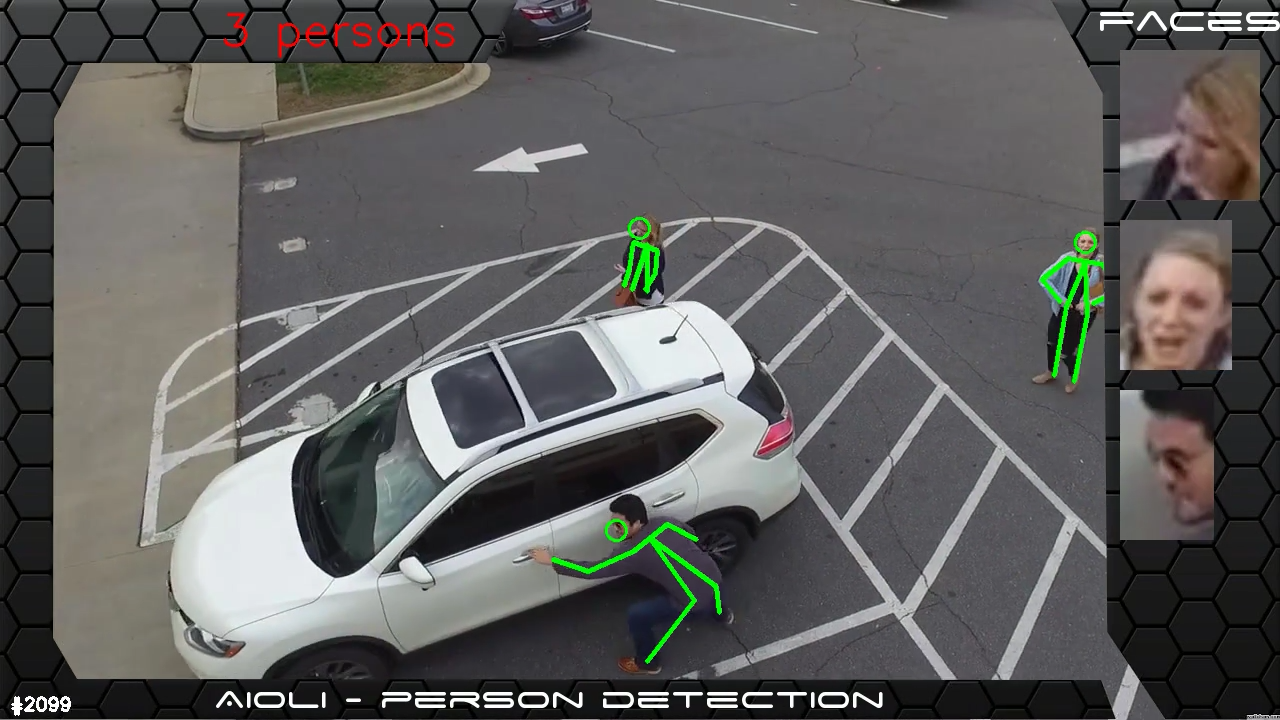
\includegraphics[width=.55\linewidth]{images/aioli_detections.png}
\end{frame}

\begin{frame}{Demo}
\centering
            \href{run:./videos/aioli_detections.mp4?autostart}
            {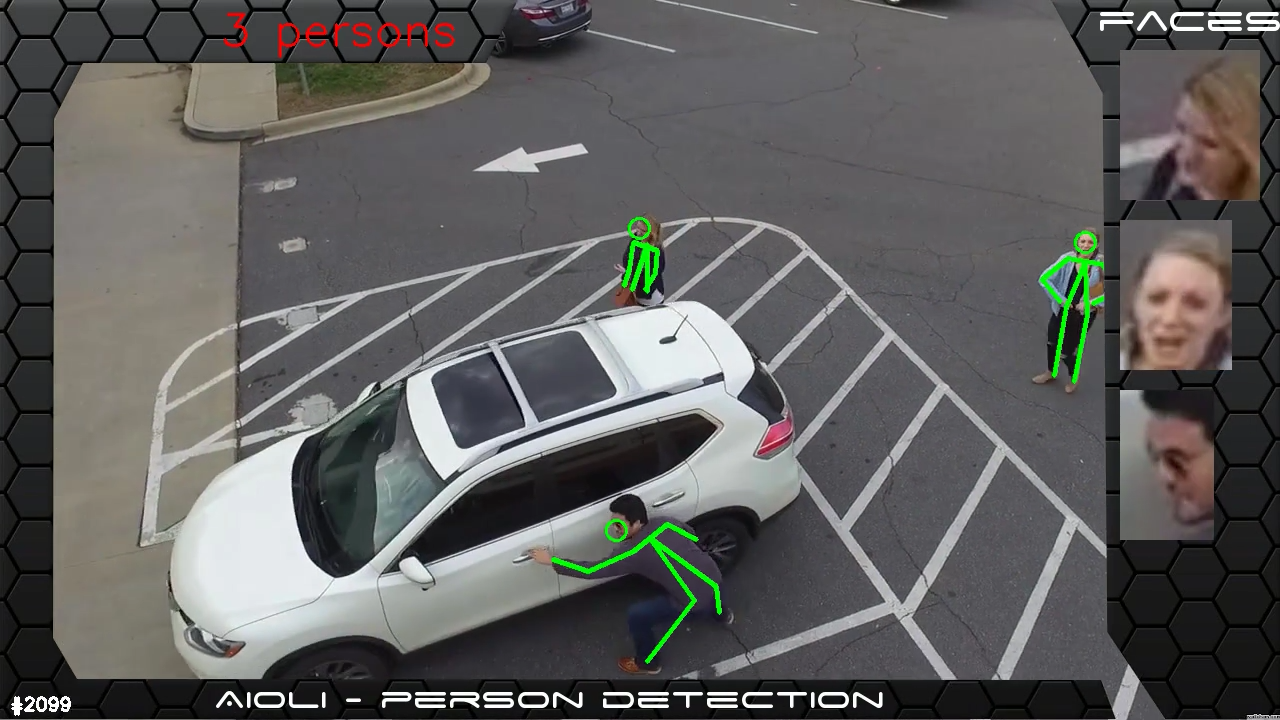
\includegraphics[width=.95\linewidth]{images/aioli_detections.png}}
\end{frame}

\begin{frame}{Detection}
	\begin{itemize}
		\item Identification requires some (most times: a lot) images of the target
		\item Famous persons: easy
		\item Others: facebook, social media, government database
		\item Current best: 83.29\% among 1Million faces on MegaFace (5 million photos, 600k persons, mean: 7pics/person)
	\end{itemize}
	\hspace{1.5cm}
	
\includegraphics[width=.3\textwidth]{images/mosaic_tobi.png}
	\hspace{1cm}
    \href{run:./videos/face_recog_new.mp4?autostart}
    {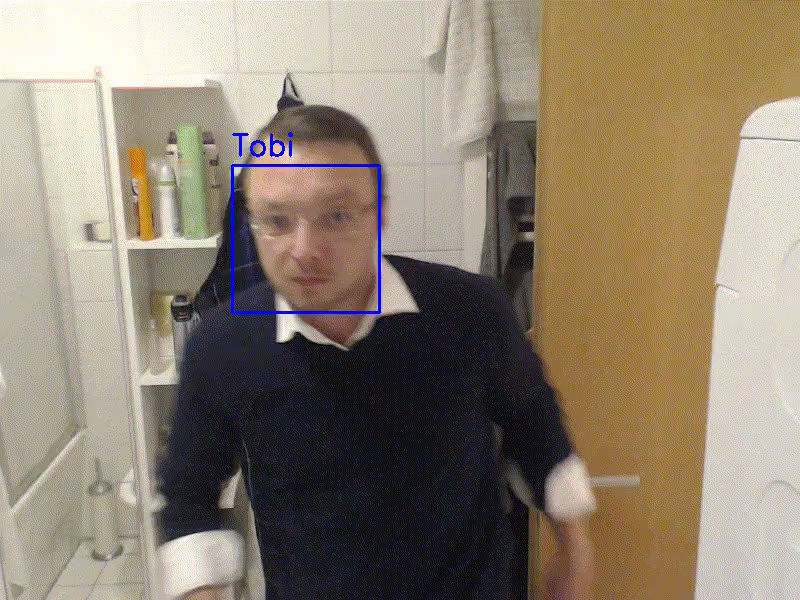
\includegraphics[width=.4\linewidth]{images/face_recog.png}}	
\end{frame}

\begin{frame}{Hardware used for this demo}
	Processed offline:
	\begin{itemize}
		\item Hardware used: NVIDIA GTX 1080 Ti, i7-7700K @ 4.2Ghz
		\item Framerate achieved: 20fps
		\item Energy spent? (GPU: 250W, @12V -> ca. 20A)
	\end{itemize}
\end{frame}

\begin{frame}{Embedded GPUs}
	\begin{columns}
		\begin{column}{.6\linewidth}
			NVIDIA Jetson TX2
			\begin{itemize}
				\item System-on-module
				\item 256-core NVIDIA Pascal GPU
				\item hex-core ARMv8 64-bit CPU
				\item 8GB of LPDDR4 memory with a 128-bit interface
				\item weight: 85g, size: 50x87mm
				\item up to 12W power consumption (@12V $\rightarrow$ 1A)
				\item Reported fps for pose-detection: 8fps
			\end{itemize}
		\end{column}
		\begin{column}{.4\linewidth}
			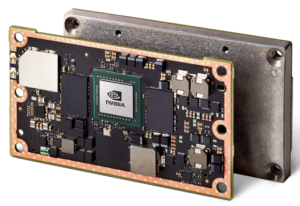
\includegraphics[width=\textwidth]{images/jetson_tx2.png}
		\end{column}
	\end{columns}
	\vspace{5mm}
			\tiny{\color{gray}{https://devblogs.nvidia.com/parallelforall/jetson-tx2-delivers-twice-intelligence-edge/}}\\
			\tiny{\color{gray}{https://github.com/CMU-Perceptual-Computing-Lab/openpose/pull/245}}	
\end{frame}

\begin{frame}{Lifting capabilites of some consumer drones}
	\begin{tabular}{|c|c|c|c|c|c|}
		\hline
		\textbf{Model} & \textbf{Payload} & \textbf{Size} & \textbf{Airtime} & \textbf{Price} & \textbf{Image}\\
		\hline
		Cheerson CX10 & 4-6g & 40x40mm, 15g & 5-8min &  15 EUR & \raisebox{-7mm}{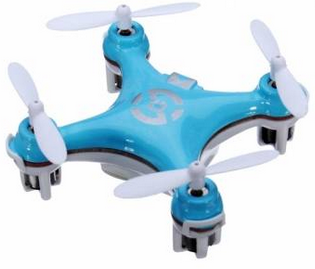
\includegraphics[height=10mm]{images/cheerson_cx10.png}}\\
		\hline
		Syma x8c & 200g & 50x50cm, 500g  &  12min & 70 EUR & \raisebox{-7mm}{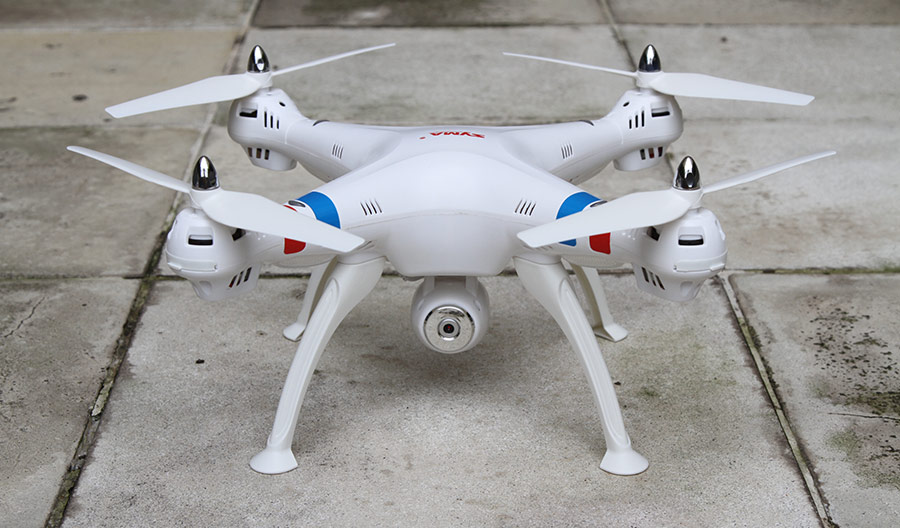
\includegraphics[height=10mm]{images/symax8c.jpg}} \\
		\hline
		3DR X8+ & 1kg & 35x50cm, 2.5 kg & 15min & 1150 EUR & \raisebox{-7mm}{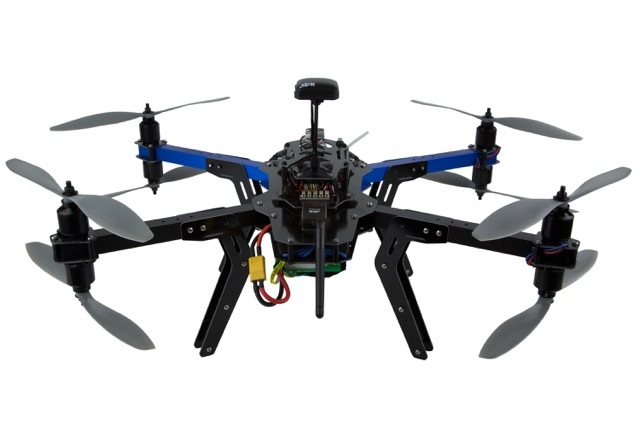
\includegraphics[height=10mm]{images/x8plus.jpeg}} \\
		\hline 
		DJI S900 & 3kg & 90cm diam, 3.3kg & 18min & 1200 EUR & \raisebox{-7mm}{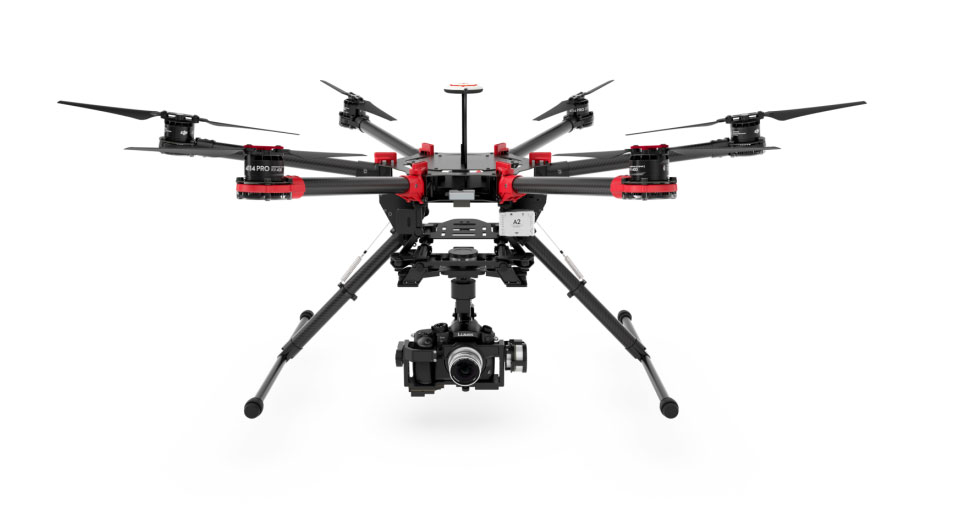
\includegraphics[height=10mm]{images/djis900.jpg}}\\
		\hline
		Tarot T18 & 8kg & 127cm diam, 8kg & 30min & 2000 EUR & \raisebox{-7mm}{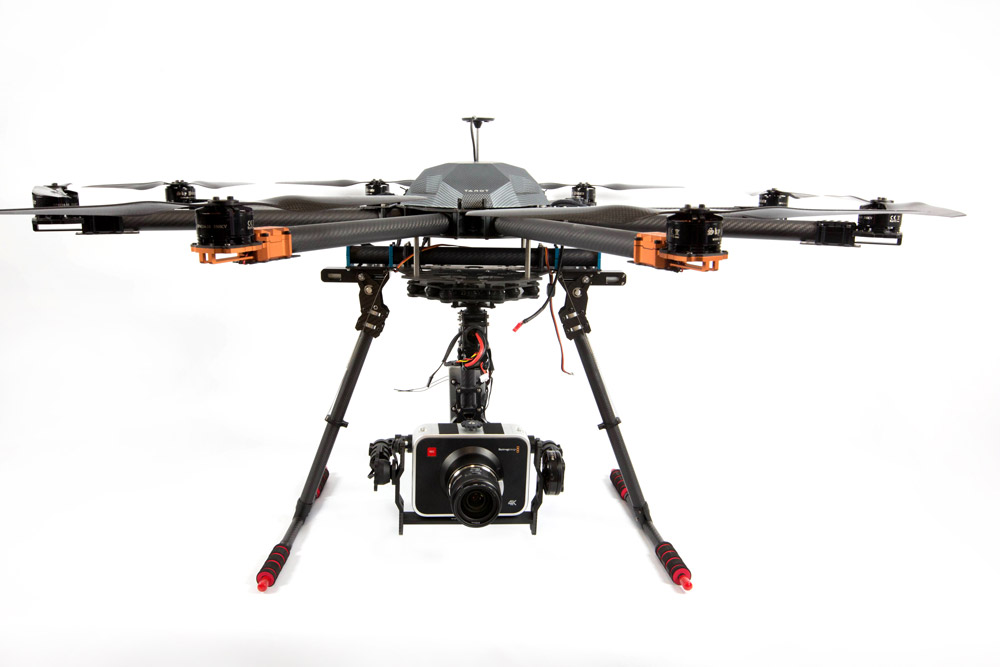
\includegraphics[height=10mm]{images/tarot18.jpg}} \\
		
		\hline
	\end{tabular}
\end{frame}

\section{Assessment}
\begin{frame}{Assessment and basis for discussions}
	Today not feasible (at least not in the complete package)
	\begin{itemize}
		\item Tradeoff between necessary compute-power, take-off-weight, flight-time, size and speed
		\item $\rightarrow$ Today not feasible in the shown size
		\item Limited flight time and range - if specific persons should be targeted, need a GPS-fix or initial position beforehand
		\item Far too expensive to be widely deployed (today: several hundred dollars)
	\end{itemize}
\end{frame}

\begin{frame}{Try it yourself}
	Want to get your hands dirty?
	\begin{itemize}
		\item Microsoft airsim Unreal simulator, c++ and python programmable: https://github.com/Microsoft/AirSim\\
		\centering
            \href{run:./videos/AirSimDemo.mp4?autostart}
            {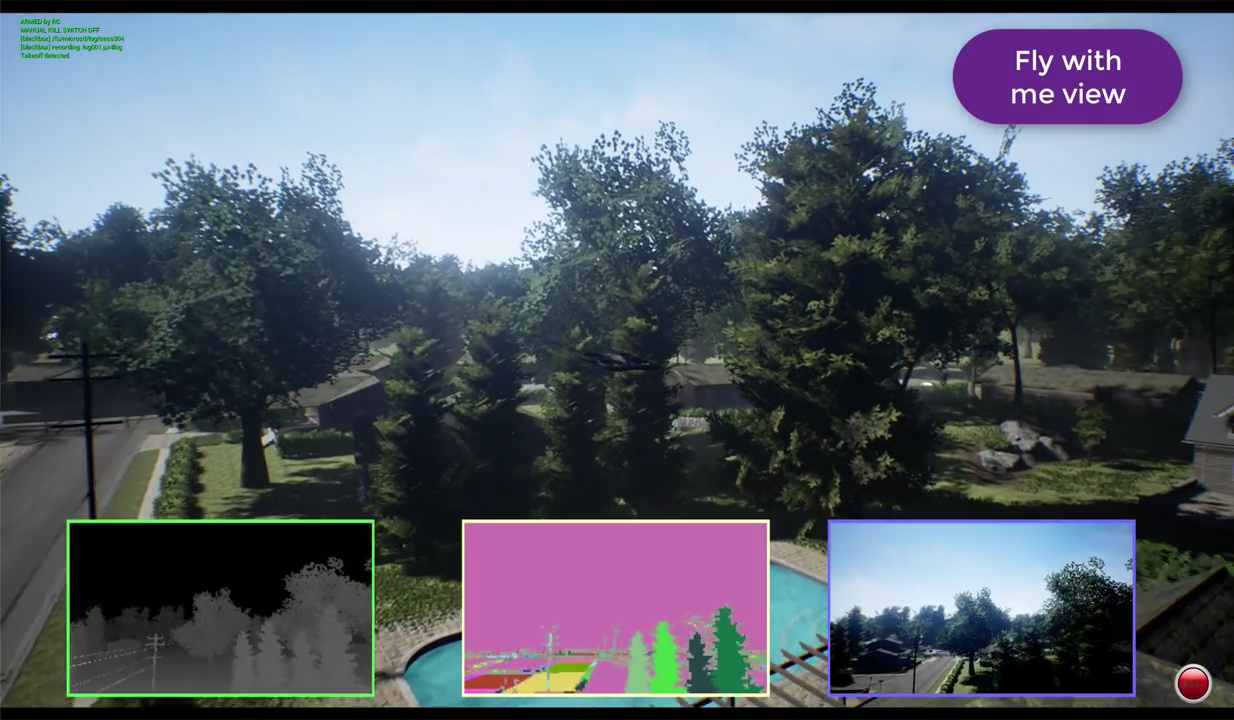
\includegraphics[width=.45\linewidth]{images/AirSimDemo.png}}	
		\item Cheap indoor, python-programmable computer vision Wifi drone: Parrot AR 2.0 (used for 50EUR on ebay)
		\item Self-built drone-plattforms with necessary parts (radio-control, camera, batteries, charger, etc.): starting from 400EUR
	\end{itemize}
\end{frame}

\begin{frame}{Discussion - End}
	\center
	\huge{Thanks a lot for your attention!}
\end{frame}

\end{document}
